\PassOptionsToPackage{table}{xcolor}
\documentclass[AMA,STIX2COL]{WileyNJDv5}

% ---------------- Packages ----------------
\usepackage{etoolbox}
\usepackage{geometry}
\usepackage{enumitem}
\usepackage{alltt}
\usepackage{fontspec}
\usepackage{tabularx}
\usepackage{booktabs}
\usepackage{ragged2e}
\usepackage{makecell}
\usepackage{xcolor}                          % <-- ADD THIS
\usepackage{array}
\newcolumntype{Y}{>{\RaggedRight\arraybackslash}X}
\usepackage[font=small]{caption}
\usepackage{tikz}
\usepackage{float}
\usepackage[most]{tcolorbox}
\usepackage{minted}
\usepackage{hyperref}
\hypersetup{hidelinks}

% ---------------- Fonts ----------------
\setmonofont{JetBrains Mono}

% ---------------- Spacing ----------------
\renewcommand{\baselinestretch}{0.9}

% ---------------- Colors ----------------
\definecolor{codebg}{gray}{0.98}
\definecolor{clsbg}{gray}{0.9}
\definecolor{Maroon}{RGB}{128,0,0}
\definecolor{darkyellow}{RGB}{218,165,32}

% ---------------- Custom commands ----------------
\newcommand{\IT}{{\sffamily EZR}}

% Class name highlight: \cls{Data}, \cls{Num}, etc.
\newcommand{\cls}[1]{%
  \setlength{\fboxsep}{1.5pt}%
  \colorbox{clsbg}{\sffamily\bfseries{#1}}%
}

% Solid disc marker: \disc{1} (black) or \disc[red]{2}
\newcommand{\disc}[2][black]{%
  \tikz[baseline=(c.base)]%
    \node[circle, fill=#1, draw=#1,
          inner sep=0pt, minimum size=1.2ex,
          text=white, font=\tiny\bfseries]
    (c) {#2};%
}

% Toggle for \rc markers (red <-> black)
\newtoggle{rcred}
\toggletrue{rcred}
\newcommand{\rctoggle}{\iftoggle{rcred}{\togglefalse{rcred}}{\toggletrue{rcred}}}
\newcommand{\rc}[1]{%
  \iftoggle{rcred}{\disc[red]{#1}}{\disc[black]{#1}}%
}

% "Hence" callout box for lesson banners
\newtcolorbox{hence}[1]{
  enhanced, breakable,
  colback=gray!5, colframe=black!70,
  fonttitle=\bfseries, coltitle=white,
  title=#1,
  left=5pt, right=5pt, top=4pt, bottom=4pt,
  boxrule=0.5pt, arc=2pt,
}

% ---------------- Minted setup ----------------
\captionsetup[listing]{skip=0pt,position=top}
\setminted{
  fontsize=\fontsize{6.5}{7.5}\selectfont,
  bgcolor=codebg,
  frame=none,
  framerule=0.5pt,
  rulecolor=\color{gray},
  framesep=2mm,
  xleftmargin=0pt,
  numbersep=2mm,
  linenos,
  firstnumber=last,
  baselinestretch=0.95,
  breaklines=true,
  breakanywhere=true,
  autogobble=true,
  escapeinside=||,
}
\setminted[python]{style=bw}
\renewcommand{\theFancyVerbLine}{%
  \color{gray}\fontsize{4}{4}\selectfont\arabic{FancyVerbLine}}
\newminted[repl]{python}{linenos=false,firstnumber=last}

% Keep minted blocks from breaking across columns
\BeforeBeginEnvironment{minted}{\par\nopagebreak\minipage{\linewidth}}
\AfterEndEnvironment{minted}{\endminipage\par\noindent}

% ---------------- Wiley journal metadata ----------------
\articletype{Research Paper}
\received{Date Month Year}
\revised{Date Month Year}
\accepted{Date Month Year}
\journal{Software: Practice and Experience}
\volume{00}
\copyyear{2026}
\startpage{1}

\begin{document}

\title{Can AI be Easy? Lessons Learned from the EZR.py    Toolkit}

\author[1]{Tim Menzies}
\author[2]{Srinath Srinivasan}

\authormark{MENZIES \textsc{et al.}}
\titlemark{Is Simple Also Stupid? Lessons from EZR}

\address[1]{\orgdiv{Department of Computer Science},
            \orgname{North Carolina State University},
            \orgaddress{\state{North Carolina}, \country{USA}}}
\address[3]{\orgdiv{Department of Computer Science},
            \orgname{North Carolina State University},
            \orgaddress{\state{North Carolina}, \country{USA}}}

\corres{Tim Menzies, \email{timm@ieee.org}}

\abstract[Abstract]{
\renewcommand{\baselinestretch}{0.9}
Much recent press claims that humans need not read code. We disagree and argue that there is much to learn by humans who  read code.
For example, EZR is a 500-line Python toolkit (no heavy dependencies) for active
learning, classification, multi-objective optimization, regression-tree
explanation, and text mining
(EZR installs via \texttt{pip install ezr}, with example data at
\texttt{github.com/timm/moot}).
EZR was built by repeatedly
reading and refactoring some AI tools in order to simplify and unify them. 

 EZR teaches us  that    many seemingly different learning algorithms are
nearly the same once stripped back to their  core: the incremental maintenance of distributions stored in
numeric and symbolic columns. Once that is coded, Na\"ive
Bayes takes two functions; k-means is thirteen lines long;  k-means++, is eleven lines; (1+1)-EAs,
need fifteen lines; the TWCNB complementary learner (for low-frequency data) is 30 lines long; and a
state-of-the-art active learner can be code in  just 35 lines.  Despite their small size, these tools performs as
good or better than state-of-the-art explanation tools (SHAP/LIME),
optimizers (SMAC/TPE), and text-mining tools (FASTREAD)---while running
10{,}000$\times$ faster and requiring orders of magnitude less labelled
data.

Based on the EZR expeience, we suggest that  (a)~AI's next step might not be larger systems but smaller, unified
ones---toolkits compact enough to be configured, critiqued, taught, and
maintained by the humans who use them;
and (b)~the way to find that next generation
of AI tools is read, very closely, the code base of our current
systems.
}

\keywords{Active learning; explanation; multi-objective
optimization; Complement Na\"ive Bayes; software analytics;
minimalism; reproducibility; literate programming}

\jnlcitation{\cname{%
\author{Menzies T.},
\author{Srinath Srinivasan}},
\ctitle{Easier AI: Lessons learned from the EZR.py    Toolkit}.
\cjournal{\it Software: Practice and Experience.}
\cvol{2026;00(00):1--20}.}

\maketitle
\section{Introduction}
\label{sec:intro}

Recently it has been argued that humans no longer need
to read code. Ryan Dahl (creator of  Node.js) suggests  that the era
of human-written code is ending~\cite{dahl2024}. Jensen Huang (Nvidia CEO) advises against
learning to code~\cite{huang2024}. Elon Musk said traditional coding ends in 2026~\cite{musk2026}.
Replit's CEO told students to focus on how to talk to machines,
not how to program~\cite{masad2025}. 
While the phrasing varies,
the argument is the same:
AI is the new compiler, and we do not read what a compiler
emits.
 


We disagree. Reading code is useful. Refactoring code is more
useful. Important low-level information  ``on the ground'' (as it were)  gets missed when developers always use LLMs to  ``fly over'' the details.

As evidence of that claim, this paper reports on \IT{}, a Python toolkit
of about 500 lines for AI in software engineering. \IT{} grew
across several years of repeatedly reading and rewriting and refactoring (we read   
  the code, looking for  similarities across distant parts of the
system, and deleting what those similarities made redundant). The
result was a small, very fast, dependency-light tool. On 120-plus
multi-objective tasks  shown in
Figure~\ref{mootdata} from the MOOT
repository~\cite{menzies2025moot}, \IT{} builds effective models
from fewer than 100 labels. It produces effective regression  trees that use
fewer than ten variables, even when thousands are available. It
runs in milliseconds. Model updates are 10{,}000 times faster
than state-of the art optimizers (SMAC~\cite{lindauer2022smac3}).







\begin{table*}[!t]
{\fontsize{7}{8}\selectfont
\setlength{\tabcolsep}{3pt}
\renewcommand{\arraystretch}{1.15}
 

\caption{The 124 multi-objective tasks in the MOOT
repository~\cite{menzies2025moot} used in this paper. Tasks are expressed as tabular daa.
Each row
is a task category. \#y is the number of goal columns; \#x is
the range of independent attribute.
Data comes from recent papers from
the SE literature (ICSE, FSE, TSE,
IST, EMSE, TOSEM, and ASE\cite{Amiraliminimaldata,chen2026promisetune,senthilkumar2024can,chen2025accuracy,lustosa2024learning,lustossa2024isneak,chen2018beyond,nyagami_fc25_kaggle_2025,blastchar_telco_customer_churn_2025,kumarajarshi_life_expectancy_who_2025,jackdaoud_marketing_data_2022}). }

\label{mootdata}
\begin{center}
\begin{tabularx}{.8\textwidth}{@{} r l l l Y c c r l @{}} 
\textbf{\#}
  & \textbf{Category}
  & \textbf{Focus}
  & \textbf{File name(s)}
  & \textbf{Optimization challenge}
  & \textbf{\#y}
  & \textbf{\#x}
  & \textbf{Rows}
  & \textbf{Refs} \\
\midrule

\multicolumn{9}{@{}l}{%
  \cellcolor{gray!25}\textbf{Software systems, configuration, and tuning}} \\
24 & Soft.\ config  & PLE     & SS-[A-X]         & Minimize footprint/memory vs.\ maximize throughput   & 2--3 & 3--88   &      197--86k & \cite{Amiraliminimaldata} \\
12 & PromiseTune    & Perf.   & 7z, LLVM, BDBC   & Minimize execution time and energy consumption       & 1    & 6--35   &     864--166k & \cite{chen2026promisetune} \\
 1 & Cloud compute  & Tuning  & Apache\_AllMeas  & Balance server response vs.\ CPU/RAM load            & 1    & 9       &           192 & \cite{senthilkumar2024can} \\
 1 & Cloud compute  & Tuning  & SQL\_AllMeas     & Minimize latency/IO vs.\ maximize throughput         & 1    & 39      &      4{,}654  & \cite{chen2025accuracy} \\
 1 & Cloud compute  & Tuning  & X264\_AllMeas    & Optimize encoding parameters for PSNR/SSIM           & 1    & 16      &      1{,}153  & \cite{Amiraliminimaldata} \\
 2 & Testing        & Testing & test120, test600 & Maximize coverage while minimizing execution time    & 1    & 9       &      5{,}161  & \\

\addlinespace[3pt]
\multicolumn{9}{@{}l}{%
  \cellcolor{gray!25}\textbf{Project management and process modeling}} \\
35 & Proj.\ health  & Health  & Health-Closed    & Optimize PR rates and minimize developer churn       & 2--3 & 5       &     10{,}001  & \cite{lustosa2024learning} \\
 3 & Scrum          & Agile   & Scrum[1k--100k]  & Maximize velocity within sprint constraints          & 3    & 124     &      1k--100k & \cite{lustosa2024isneak} \\
 8 & Feature mod.   & Config  & FFM, FM-*        & Optimize clause/constraint ratio in large spaces     & 3    & 128--1k &     10{,}001  & \cite{Amiraliminimaldata} \\
 1 & nasa93dem      & Cost    & nasa93dem        & Minimize effort (person-months) vs.\ quality         & 3    & 26      &            93 & \cite{lustosa2024learning} \\
 1 & COC1000        & Risk    & coc1000          & Minimize risks vs.\ analyst expertise                & 5    & 20      &      1{,}001  & \cite{chen2018beyond} \\
 4 & POM3           & Process & pom3[a-d]        & Balance project idle rates vs.\ completion costs     & 3    & 9       &      501--20k & \cite{lustosa2024isneak} \\
 4 & XOMO           & Defects & xomo\_[flt,grd]  & Minimize defect density vs.\ total project effort    & 4    & 27      &     10{,}001  & \cite{chen2018beyond} \\

\addlinespace[3pt]
\multicolumn{9}{@{}l}{%
  \cellcolor{gray!25}\textbf{Interdisciplinary and behavioral benchmarks}} \\
 4 & Behavioral     & Behavior  & all\_players, etc.\ & Maximize user retention and predict cohort churn  & 1--3 & 26--55  &     82--17k   & \cite{nyagami_fc25_kaggle_2025} \\
 4 & Financial      & Finance   & BankChurners      & Minimize credit risk vs.\ pricing models            & 2--5 & 19--77  &      1k--20k  & \cite{blastchar_telco_customer_churn_2025} \\
 3 & Health         & Health    & COVID19, Life     & Maximize accuracy/life vs.\ readmission likelihood  & 1--3 & 20--64  &      2k--25k  & \cite{kumarajarshi_life_expectancy_who_2025} \\
 2 & RL             & Control   & A2C\_[Acr,Crt]    & Maximize reward signals vs.\ steps to convergence   & 3--4 & 9--11   &      224--318 & \\
 5 & Sales          & Market    & Marketing, socks  & Maximize ROI vs.\ minimize forecasting error        & 1--8 & 20--31  &       247--2k & \cite{jackdaoud_marketing_data_2022} \\
 3 & Misc.          & General   & auto93, Car       & Optimize multivariate trade-offs (e.g.\ MPG vs.\ HP) & 2--5 & 5--38   &       205--1k & \cite{Amiraliminimaldata} \\

\midrule
\textbf{124 } & \multicolumn{8}{@{}l}{\textbf{total}}  
\end{tabularx}
\end{center}
}
\end{table*}


% These properties are useful. The methodological claim is
% different. We found these properties by reading the code. The
% smallness of the data, the smallness of the models, and the
% smallness of the code are facets of one finding: AI systems for
% SE contain more redundancy than is generally assumed, and
% removing the redundancy leaves something surprisingly small.
 

From this work, we draw  five lessons.
After some preliminaries, this paper
is structured around these   lessons.


\begin{itemize}
\item In \S\ref{sec:peek}, \S\ref{sec:famous}, and
\S\ref{sec:active}, we show that a handful of data structures
suffices to code a wide range of AI tools. Classification,
clustering, optimization, regression, active learning, and text
mining all ride on the same incremental
\cls{Num}/\cls{Sym}/\cls{Data} substrate.

\item In \S\ref{sec:famous} and \S\ref{sec:opt}, we show that
optimization, classification, and regression are nearly the same
algorithm. What looks in the textbook like separate fields is, in
code, repeated use of one substrate.

\item In \S\ref{sec:opt}, we show that random search works better
than expected. Three classical optimizers (simulated annealing,
local search, (1+1)-EA) are statistically indistinguishable on
MOOT. They differ only in a one-line accept rule.

\item In \S\ref{sec:active}, we show that the same substrate
yields an active learner that runs 10{,}000$\times$ faster than
SMAC while matching its solution quality, using O(1) incremental
updates instead of tree-ensemble refits.

\item In \S\ref{sec:tiny} and \S\ref{sec:valid}, we show that
many models can be tiny. Across 120-plus MOOT tasks, fewer than
ten variables suffice even when thousands are available---and
held-out validation shows these small trees travel: a few
oracle calls at deployment time reach 85--95\% of the reference
optimum.

\item In \S\ref{sec:textmine}, we show that 30 lines of TWCNB on
the same substrate matches FASTREAD's relevance-filtering
results on three of four SLR corpora, using one-seventh the
labels---and exposes a measurement gap (false alarm) the
original study did not report.

\item Overall, we show that small codebases work. EZR is
500 lines, runs in milliseconds, and has no heavy dependencies,
which means less supply-chain risk, easier review, faster
porting, and more visible structure for the next round of
refactoring.
\end{itemize}

 Each of these claims invites the same objection: that simple is
stupid. High-dimensional problems should need many features.
SMAC's tree ensemble should beat random. Different fields have
different textbooks for a reason. Real work needs pandas and
scikit-learn. The body of this paper offers evidence to the
contrary, lesson by lesson, with code in front of you so the
claims can be audited.

\subsection*{The empirical record}

Across two prior studies, \IT{} has matched state-of-the-art
explanation tools (SHAP, LIME, Anchors)~\cite{amirali} and
multi-objective optimizers (SMAC, TPE,
HyperOpt)~\cite{kashin}. \IT{} did so while using 10 to 10{,}000
times less code, less data, and less compute. This paper extends
that record. We applied \IT{} to reanalyze a prior text-mining
study from Yu et al.~\cite{yu2018finding} on relevance filtering
for systematic literature reviews. The simplification went
further. Thirty lines of TWCNB, riding on the same substrate,
matched Yu's results with roughly one-seventh of the labels. The
analysis also surfaced a finding the original study could not
have made because it did not measure false alarm.

So: three independent comparisons, three domains, the same
pattern. Simple, when carefully built, is not stupid. The rest
of this paper documents how the substrate makes that pattern
possible, and what habits of attention we had to develop to find
it.

\subsection*{Caveat}

Not all AI tasks can be simplified this way. Generative tasks
including translation, summarization, and natural-language
interfaces need LLMs and the data scales that come with them.
We do not argue that LLMs are unnecessary. We argue that many
SE tasks (configuration, tuning, defect prediction, testing,
cost estimation, relevance filtering) admit much simpler
solutions. These are often, more often than the field
acknowledges, already sufficient. The right move is to try the
simple thing first. Even when it is later outperformed, the
simple thing sets a strict performance floor (so you can
measure exactly what the complex model adds) and provides
transparency a black-box model cannot.

\section{A Peek at the Code}\label{sec:peek}

This section introduces the substrate that the rest of the
paper relies on. Four classes carry almost everything. \cls{Num}
and \cls{Sym} summarize columns of numbers and symbols.
\cls{Data} holds rows summarized by those columns. \cls{Cols}
is a small factory that builds the columns from a CSV header.
One function, \textsf{add}, walks all four polymorphically and
is the only way data ever enters the system. The substrate is
small enough to hold in your head. That smallness is what later
sections exploit.

A few stylistic points before the code. Per Martin's clean-code
rules~\cite{martin2009clean} (write functions small, then
smaller still), \texttt{ezr.py}'s 44 functions average $5\pm4$
lines. Each line is under 60 characters wide so it can be
included in documents like this one without reformatting.
Following Hatton~\cite{Hatton:1998}, \IT{} avoids inheritance
because inheritance complicates functional
composition~\cite{GoF:1995} and debugging~\cite{hatton1998oo}.
Polymorphism is implemented by casing on type inside functions.
\IT{} prefers functions over methods. Methods scatter related
code across classes; functions let related code group together.
The \textsf{mid} and \textsf{spread} pair below is one example.

To dodge supply-chain risk, \IT{} uses few imported packages.
Modern Python software is often assembled from pre-made parts,
with 85 to 97 percent of code reused from external
sources~\cite{martinez2021}. Libraries like \texttt{pandas} are
battle-tested but introduce a large attack surface. A single
poisoned update can compromise tens of thousands of downstream
packages without the primary developer's
knowledge~\cite{martinez2021}. \IT{} ships with one CSV reader
of 14 lines:

\begin{minted}{python}
def csv(f, clean=lambda txt:
          txt.partition("#")[0].split(",")):
  """Yield typed rows from a CSV file."""
  with open(f, encoding="utf-8") as file:
    for txt in file: |\label{csv}|
      row = clean(txt)
      if any(x.strip() for x in row):
        yield [thing(x) for x in row]

def thing(txt):
  """Coerce string to number or bool."""
  txt = txt.strip()
  b = lambda s: {"true":1,"false":0}.get(
                  s.lower(), s)
  for f in [int, float, b]:
    try: return f(txt)
    except ValueError: pass
\end{minted}

The reader skips comments after \texttt{\#}, splits on commas,
yields typed rows. \textsf{thing} coerces each cell to int,
float, bool, or string in turn. Pandas does more, at the cost
of around half a million lines of dependency. The 14 lines
above do exactly what \IT{} needs.

\subsection{An example CSV}

\IT{} reads tabular data with a small set of column-name
conventions. Names ending in ``X'' are ignored (e.g.\ row IDs
or timestamps). Names ending in ``!'' mark a symbolic class
column. Names ending in ``+'' or ``-'' mark goal columns to be
maximized or minimized. Everything else is an independent
attribute. Numeric columns start with an upper-case letter;
symbolic columns do not.

Table~\ref{moot} shows a typical example. The data come from a
configuration-tuning task in the MOOT
repository~\cite{menzies2025moot}, which is the benchmark used
later in this paper. The header tells \IT{} everything it
needs. \texttt{Spout\_wait} starts with an upper-case letter,
so it is a \cls{Num}. \texttt{Spliters} and \texttt{Cntr} also
start uppercase, so they are \cls{Num}s as well.
\texttt{Throughput+} ends in ``+'', so \texttt{Throughput} is to
be maximized. \texttt{Latency-} ends in ``-'', so
\texttt{Latency} is to be minimized.

\begin{table}[!t]
\caption{An example MOOT data set: configuration tuning for a
distributed stream-processing system. Numeric column names
start with an upper-case letter. Goal column names end with
``+'' (maximize) or ``-'' (minimize). Everything else is an
independent attribute.}
\label{moot}
\begin{center}
\begin{minipage}{3in}
\normalsize{(a) Configuration tuning:}
{\fontsize{6pt}{7.2pt}\selectfont

\begin{verbatim}
x = independent values      | y = dependent values
----------------------------|-----------------------
Spout_wait, Spliters, Cntr. | Throughput+, Latency-
    10,        6,       17  |    23075,    158.68
     8,        6,       17  |    22887,    172.74
     9,        6,       17  |    22799,    156.83
[Skipped],  ...,      ...   |       ...,      ...
 10000,        1,       10  |    460.81,    8761.6
 10000,        1,       18  |    402.53,    8797.5
 10000,        1,        1  |    310.06,    9421
-------------------------------------------------------
\end{verbatim}}
\normalsize{(b) Defect prediction}
{\fontsize{6pt}{7.2pt}\selectfont
\begin{verbatim}
x = independent values    | y = dependent values
--------------------------|---------------------
Numobs, Length, ..., Churn| Class+
 3317,   2990, ...,  0.2  |   1
 5873,   1923, ...,  0.4  |   2
 2357,   1333, ...,  0.0  |   2
[Skipped],     ...,  ...  |   ...
 1104,    891, ...,  0.4  |   3
  204,     38, ...,  0.4  |   3
 1939,   1236, ...,  0.1  |   3
-------------------------------------------------------
\end{verbatim}}
\normalsize{(c) Hyperparameters for Software Health Prediction}
{\fontsize{6pt}{7.2pt}\selectfont
\begin{verbatim}
x = independent values          | y = dependent values
-------------------------------|----------------------
N_est, Min_leaf, ..., Min_imp. | MRE-, ACC+, PRED40+
   40,      1,    ...,    0.25 | 0.205, 0.826, 1.00
  120,      1,    ...,    4.75 | 0.191, 0.756, 1.00
   10,      1,    ...,    6.75 | 0.000, 0.790, 0.86
[Skipped],      ...,    ...    |   ...,   ...,   ...
   10,     11,    ...,    5.25 | 0.925, 0.391, 0.00
   90,     12,    ...,    5.00 | 0.911, 0.397, 0.00
  130,      9,    ...,    9.75 | 0.914, 0.395, 0.00
\end{verbatim}}
\end{minipage}
\end{center}
\end{table}

\subsection{Columns: \cls{Num} and \cls{Sym}}

\IT{} distinguishes numeric and symbolic columns. Both know
their text name (\textsf{txt}), their position in the row
(\textsf{at}), and how many items they have seen (\textsf{n}).

\cls{Num}eric columns track a running mean (\textsf{mu}), a
second moment (\textsf{m2}), a standard deviation (\textsf{sd},
derived from \textsf{m2}), and a \textsf{heaven} value
indicating goal direction. By convention, columns whose names
end in ``+'' are to be maximized and columns whose names end in
``-'' are to be minimized. \textsf{heaven} is set to 1 or 0
respectively. Smaller distance to \textsf{heaven} is always
better.

\begin{minted}{python}
class Num:
  """Summarizes a stream of numbers."""
  def __init__(i, txt="", at=0):
    i.txt, i.at, i.n = txt, at, 0
    i.mu = i.m2 = i.sd = 0
    i.heaven = txt[-1:] != "-" |\label{heaven}|
\end{minted}

\cls{Sym}bolic columns hold frequency counts in a \textsf{has}
dictionary:

\begin{minted}{python}
class Sym:
  """Summarizes a stream of symbols."""
  def __init__(i, txt="", at=0):
    i.txt, i.at, i.n, i.has = txt, at, 0, {}
\end{minted}

This pair is small. It is enough to support central-tendency,
variability, and normalization queries by polymorphism on type.
The \textsf{mid} of a column is its mean for numbers and its
mode for symbols:

\begin{minted}{python}
def mid(col):
  return (col.mu if Num==type(col)
          else mode(col.has))

def mode(dct): return max(dct, key=dct.get)
\end{minted}

The \textsf{spread} is its standard deviation for numbers and
its entropy for symbols:

\begin{minted}{python}
def spread(col):
  return (col.sd if Num==type(col)
          else entropy(col.has))

def entropy(dct):
  n = sum(dct.values())
  return -sum(v/n*log2(v/n)
              for v in dct.values())
\end{minted}

The textbook treats this as four formulas. \IT{} treats it as
one question (``summarize this column'') asked of two types.

Numeric values can also be normalized to $[0,1]$ via a logistic
sigmoid clamped to $\pm3$ standard deviations. Missing values
(``?'') pass through:

\begin{minted}{python}
def norm(num, v):
  if v == "?": return v
  z = (v - num.mu) / (num.sd + 1e-32)
  z = max(-3, min(3, z))
  return 1 / (1 + exp(-1.7*z))
\end{minted}

\textsf{norm} makes rows from different scales comparable for
distance calculations later in the paper.

\subsection{Rows and tables: \cls{Data} and \cls{Cols}}

\cls{Data} holds rows together with summarized columns. Its
constructor accepts an iterator (e.g.\ from \textsf{csv}) or a
list of rows. The first row becomes the header and is handed
to \cls{Cols} to build the column objects. The rest are added
in turn:

\begin{minted}{python}
class Data:
  """Rows + summarized columns."""
  def __init__(i, src=None):
    src = iter(src or {})
    i.rows, i._centroid = [], None
    i.cols = Cols(next(src))
    adds(src, i)
\end{minted}

Two usage patterns appear throughout:

\begin{repl}
>>> data1 = Data(csv(fileName))           # from disk
>>> data2 = Data([data1.cols.names])      # empty clone
\end{repl}

The second pattern (an empty \cls{Data} that mimics another's
column structure) is wrapped in a helper:

\begin{minted}{python}
def clone(data, rows=None):
  """Clone column structure; optionally fill with rows."""
  return adds(rows or [], Data([data.cols.names]))
\end{minted}

\textsf{clone} appears nine times in the rest of
\texttt{ezr.py}. Each appearance spawns a fresh \cls{Data} that
shares its parent's schema. Once \textsf{clone} exists, you
stop thinking about column types. You ask \cls{Data} for an
empty copy and start filling it.

\cls{Cols} is the factory that reads the header. Recall the
column-name conventions: names ending in ``X'' are ignored,
``!'' marks a symbolic class column, ``+'' or ``-'' mark goal
columns (\textsf{ys}), everything else is an independent
attribute (\textsf{xs}). Names starting with an upper-case
letter become \cls{Num}; everything else becomes \cls{Sym}.

\begin{minted}{python}
def Col(txt="", a=0):
  return (Num if txt[:1].isupper()
          else Sym)(txt, a)

class Cols:
  """Organize Num/Sym columns from headers."""
  def __init__(i, names):
    i.names = names
    i.klass, i.xs, i.ys, i.all = None, [], [], []
    for j, txt in enumerate(names):
      i.all.append(col := Col(txt, j))
      if txt[-1] != "X":
        if txt[-1] == "!": i.klass = col
        role = (i.ys if txt[-1] in "+-!"
                else i.xs)
        role.append(col)
\end{minted}

After \cls{Cols} runs, every \cls{Data} carries three views of
its columns: \textsf{xs} (independent), \textsf{ys} (dependent
goals), and \textsf{klass} (the optional symbolic target). The
rest of \texttt{ezr.py} consults these views without re-parsing
names. Decisions made once at the header propagate everywhere.

\subsection{The \textsf{add} primitive}

There is one way to put a value into the substrate: \textsf{add}.
The function dispatches on the type of its first argument and
walks recursively.

\begin{itemize}
\item Given a \cls{Data}, it invalidates the cached centroid,
recursively updates the columns, and either appends or removes
the row.
\item Given a \cls{Cols}, it walks each column and recursively
calls \textsf{add} with the appropriate cell.
\item Given a \cls{Sym}, it adds (or subtracts) one from the
\textsf{has} dictionary.
\item Given a \cls{Num}, it updates \textsf{mu}, \textsf{m2}, and
\textsf{sd} via Welford's algorithm~\cite{Knuth1998TAOCP2},
which is exact and incremental.
\end{itemize}

\begin{minted}{python}
def add(it, v, w=1):
  """Add (w=+1) or remove (w=-1) value/row."""
  if Data is type(it):
    it._centroid = None |\label{zap}|
    add(it.cols, v, w) |\label{addrec1}|
    if w>0: it.rows.append(v)
    else  : it.rows.remove(v)
  elif Cols is type(it):
    [add(col, v[col.at], w)
     for col in it.all] |\label{addrec2}|
  elif v != "?": # skip "don't know" values
    if Sym == type(it):
      it.has[v] = w + it.has.get(v, 0) |\label{symaddsub}|
    elif w < 0 and it.n <= 2:
      it.n = it.mu = it.m2 = it.sd = 0
    else: # Welford's algorithm |\label{welford}|
      it.n  += w
      delta  = v - it.mu
      it.mu += w * delta / it.n
      it.m2 += w * delta * (v - it.mu)
      it.sd  = (sqrt(max(0,it.m2)/(it.n-1))
                if it.n>1 else 0)
  return v
\end{minted}

A few details worth flagging. The \textsf{w} parameter handles
both addition (\textsf{w=1}) and subtraction (\textsf{w=-1}).
A one-line companion exposes the latter:

\begin{minted}{python}
def sub(it, v): return add(it, v, w=-1)
\end{minted}

This symmetry matters because it makes data movement cheap. A
row can be removed from one \cls{Data} and added to another
with two constant-time operations: $\pm 1$ to a counter for
symbols, or a single Welford update for numbers. There is no
retraining step. There is no resorting of large collections.
\textsf{add} and \textsf{sub} are inverses of the same
incremental update.

The cached centroid is the other detail. Centroids are
expensive when called repeatedly but cheap if cached. Every
\cls{Data} carries a \textsf{\_centroid} field that
\textsf{add} invalidates on any change (line~\ref{zap}). The
\textsf{mids} accessor lazily rebuilds it:

\begin{minted}{python}
def mids(data):
  data._centroid = data._centroid or [
    mid(col) for col in data.cols.all]
  return data._centroid
\end{minted}

Without the cache, each \textsf{mids} call would walk every
column. With it, the call is one dictionary lookup until the
next \textsf{add}.

\textsf{add} returns the value it stored. A small idiom uses
this: a value can be inserted into multiple \cls{Data}s in a
single chained call, with the inner \textsf{add} producing the
value the outer \textsf{add} consumes. The idiom appears
several times later.

\medskip

That is the substrate. Four classes, one accessor, one
mutator. The rest of the paper builds on it.


\section{Three Famous Algorithms in 30 Lines}\label{sec:famous}

\S\ref{sec:peek} promised that the rest of the paper builds on
the substrate. This section is the first instance. We show
three textbook algorithms, each given its own lecture in a
standard AI course, falling out of the substrate in well under
a hundred lines between them. Naïve Bayes takes two functions.
$k$-means takes thirteen lines. $k$-means++ takes eleven. The
algorithms are not new. The point is that once \cls{Num},
\cls{Sym}, \cls{Data}, and \textsf{add} are in place, none of
the three needs new machinery.

\subsection{Naïve Bayes in two functions}

The core of Naïve Bayes is one question: how much does a column
{\em like} a value? \textsf{like} answers that question. For a
\cls{Sym}, the answer is a smoothed frequency count from
\textsf{has} (the same dictionary \textsf{add} updates at
line~\ref{symaddsub}). For a \cls{Num}, the answer is a Gaussian
PDF using the running \textsf{mu} and \textsf{sd} that
\textsf{add} maintains via Welford (line~\ref{welford}):

\begin{minted}{python}
the.bayes.k = 1   # smoothing config

def like(col, v, prior):
  """How much a column likes a value."""
  if type(col) == Sym:
    return (col.has.get(v,0) +
            the.bayes.k*prior
           ) / (col.n + the.bayes.k)
  sd = col.sd + 1e-32
  z  = 2*sd*sd
  return exp(-(v-col.mu)**2 / z) / sqrt(pi*z)
\end{minted}

Note what is not here: no fitting pass, no separate training
phase. The \cls{Num} and \cls{Sym} columns inside a \cls{Data}
are already a fitted Bayes model, because \textsf{add} kept
them fitted incrementally as rows arrived. \textsf{like} just
reads them.

\textsf{likes} aggregates one row's worth of evidence. It
multiplies per-column likelihoods (in log space, for numerical
stability) with an $m$-estimate prior on class size:

\begin{minted}{python}
the.bayes.m = 2   # prior config

def likes(data, row, n_rows, n_klasses):
  """Log likelihood of row given data."""
  prior = (len(data.rows) + the.bayes.m
          ) / (n_rows + the.bayes.m*n_klasses)
  ls = [like(col, v, prior)
        for col in data.cols.xs
        if (v := row[col.at]) != "?"]
  return log(prior) + sum(log(v)
                          for v in ls if v > 0)
\end{minted}

That is a complete Naïve Bayes classifier with Laplace and
$m$-estimate smoothing, Gaussian numeric attributes, and
missing-value handling. Two functions. The textbook treatment
is a chapter.

To put \textsf{like} and \textsf{likes} to work, \textsf{classify}
implements the standard incremental {\em test-then-train}
protocol. Each row is first classified using the model so far
(it is assigned to the \cls{Data} with the highest
\textsf{likes} score), then added to its true class's
\cls{Data}. Because \textsf{add} is incremental, this is
genuinely streaming. No retraining. No batch passes.

\begin{minted}{python}
def classify(src, wait=10):
  """Test then train: classify before update."""
  src = iter(src)
  h, cf, all = {}, None, Data([next(src)])
  for n, row in enumerate(src):
    want = row[all.cols.klass.at]
    if n >= wait:
      cf = dinc(want, max(h,
        key=lambda kl: likes(
          h[kl], row, len(all.rows), len(h))), cf)
    if want not in h: h[want] = clone(all)
    add(all, add(h[want], row))
  return cf
\end{minted}

A few things about this loop. \textsf{wait=10} holds off scoring
until the model has seen enough rows to be worth consulting.
\textsf{dinc} accumulates a confusion matrix. \textsf{h} is a
dictionary mapping each class label to its own \cls{Data}.
\textsf{all} is the union of every class. The nested
\textsf{add(all, add(h[want], row))} uses the return-value
idiom from \S\ref{sec:peek}: the inner \textsf{add} stores
\textsf{row} into \textsf{h[want]} and returns it; the outer
\textsf{add} then stores the same row into \textsf{all}. One
row, two destinations, two function calls.

On standard MOOT classification benchmarks (soybean, diabetes,
and others), \textsf{classify} is competitive with sklearn's
batch Naïve Bayes. The substrate did most of the work.

\subsection{$k$-means in thirteen lines}

$k$-means cycles assignment and update. Assignment puts each
row into the cluster whose centroid is closest. Update recomputes
the centroid from the rows in each cluster. Both halves use
machinery that already exists. \textsf{distx} is a Minkowski
distance over independent columns:

\begin{minted}{python}
def distx(data, r1, r2):
  return minkowski(
    aha(col, r1[col.at], r2[col.at])
    for col in data.cols.xs)
\end{minted}

\textsf{mids} returns the per-column \textsf{mid} of a
\cls{Data} (line numbers below refer back to \S\ref{sec:peek}).
A cluster is just a \cls{Data} populated by \textsf{add}. So
$k$-means is:

\begin{minted}{python}
def kmeans(d, rs=None, k=10, n=10, cents=None):
  """Cluster rows into k groups."""
  rs = rs or d.rows
  cents = cents or choices(rs, k=k)
  out = []
  for _ in range(n):
    out = [clone(d) for _ in cents]
    for r in rs:
      add(out[min(range(len(cents)),
        key=lambda j: distx(d, cents[j], r))], r)
    cents = [mids(kid)
             for kid in out if kid.rows]
  return out
\end{minted}

Every primitive in this loop already existed before $k$-means
was written. \textsf{clone} (\S\ref{sec:peek}) makes the empty
cluster shells. \textsf{add} fills them. \textsf{distx}
measures membership. \textsf{mids} produces the new centroids.
$k$-means rides on the substrate without needing anything new.

\subsection{$k$-means++ in eleven lines}

The standard $k$-means++ rule says: pick one centroid at
random, then pick each subsequent centroid with probability
proportional to its squared distance from the nearest existing
centroid. The phrase ``with probability proportional to'' is
the work. Everything else is bookkeeping.

\IT{} already had that work done. \textsf{pick} samples from a
weighted distribution, and the dispatch is the same
polymorphism-by-type that \textsf{mid} and \textsf{spread} use:

\begin{minted}{python}
def pick(it, v=None):
  """Sample from distribution."""
  if Sym == type(it): return pick(it.has)
  if Num == type(it):
    tmp = (v if v is not None and v != "?"
           else it.mu)
    lo = it.mu - 3*it.sd
    hi = it.mu + 3*it.sd
    new = tmp + it.sd*2*(
            rand() + rand() + rand() - 1.5)
    return lo + (new - lo) % (hi - lo + 1e-32)
  if dict == type(it):
    n = sum(it.values()) * rand()
    for k, v in it.items():
      if (n := n - v) <= 0: return k
\end{minted}

The dict branch is a roulette-wheel sampler: accumulate random
mass, return the key where it runs out. \textsf{pick} was first
written to support synthetic-data generation in mutation
operators (used later in \S\ref{sec:opt}). The dict branch is
exactly what $k$-means++ needs.

So $k$-means++ is just: build the weight dict, sample, repeat:

\begin{minted}{python}
def kpp(d, rs=None, k=10, few=256):
  """k-means++ centroid selection."""
  rs = rs or d.rows
  out = [choice(rs)]
  while len(out) < k:
    t = sample(rs, min(few, len(rs)))
    ws = {i: min(distx(d, t[i], c)**2
                 for c in out)
          for i in range(len(t))}
    out.append(t[pick(ws)])
  return out
\end{minted}

\textsf{few=256} is a pragmatic shortcut. On large data sets,
scanning every row for each new centroid is wasteful when 256
random ones give an adequate weight distribution. The same
instinct that makes \textsf{the.few=128} sufficient for active
learning makes \textsf{few=256} sufficient here. Reading the
code surfaces this kind of cross-algorithm symmetry.

\subsection*{The lesson: one substrate, three textbooks}

Three sections of the standard AI curriculum, around 30 lines
of new code between them. None of the three needed a new data
structure. None needed a new training phase. Each is a way of
asking the substrate a different question:

\begin{itemize}
\item Naïve Bayes asks: how much does this column like this
value?
\item $k$-means asks: which centroid is this row closest to?
\item $k$-means++ asks: which row should be the next centroid,
weighted by squared distance?
\end{itemize}

The questions are different. The machinery underneath is the
same.

This is the structural similarity that recent commentary about
not reading AI code says humans no longer need to see. Without
seeing it, you write the three algorithms three times, in three
styles, with three sets of bugs. With it, you write one
substrate and reuse it. The 30-line outcome is not clever
compression. It is what is left when you read the code
carefully enough to notice that the chapters were the same
chapter all along.

\section{Three Optimizers, One Algorithm}\label{sec:opt}

\S\ref{sec:famous} did three classifiers and clusterers. We do
three optimizers here. The (1+1) evolutionary algorithm,
simulated annealing, and local search appear in textbooks as
separate methods. In \texttt{ezr.py} they are the same loop
with different one-line accept rules.

This buys us two of the lessons from \S\ref{sec:intro}. Lesson 4
says optimization, classification, and regression are nearly the
same algorithm. Lesson 2 says random search is more competitive
than the metaheuristics literature suggests. Both come out of
the same code.

One housekeeping item. Optimizers need a way to say which row is
better. We use \textsf{disty}, which is the Euclidean distance
from a row to an ideal point computed only on goal columns. From
line~\ref{heaven}, each goal column knows its ideal value: 1 for
``+'' columns, 0 for ``-'' columns. \textsf{disty} just walks the
goal columns:

\begin{minted}{python}
def disty(data, row):
  """Distance to heaven on Y vars."""
  return minkowski(
    abs(norm(col, row[col.at]) - col.heaven)
    for col in data.cols.ys)
\end{minted}

Lower scores are better. \S\ref{sec:using} expands the role of
\textsf{disty} when active learning needs it. Here a one-line
definition is fine.

\subsection{Mutation via \textsf{pick}; scoring via \textsf{nearest}}

You need three things to optimize: a way to perturb a row, a way
to score the result, and a rule for accepting the change. \IT{}
already has the first two.

\textsf{picks} mutates a row by replacing some random independent
columns with new values drawn from \textsf{pick}, the sampler we
saw in \S\ref{sec:famous} for $k$-means++. For \cls{Num} columns,
\textsf{pick} jiggles the value around a Gaussian centered near
the current value. For \cls{Sym} columns, it samples from the
observed distribution.

\begin{minted}{python}
def picks(data, row, n=1):
  """Mutate n random x-columns."""
  s = row[:]
  for col in sample(data.cols.xs,
                    min(n, len(data.cols.xs))):
    s[col.at] = pick(col, s[col.at])
  return s
\end{minted}

Scoring is harder. Running the real oracle on each candidate is
the whole reason this paper exists. We substitute a cheap
proxy: find the closest already-labeled row in $x$-space, copy
its $y$ values into the candidate, and call \textsf{disty}.

\begin{minted}{python}
def oracleNearest(data, row):
  """Score: copy y-vals from nearest labeled."""
  near = nearest(data, row)
  for col in data.cols.ys:
    row[col.at] = near[col.at]
  return disty(data, row)
\end{minted}

Three lines. This is a 1-NN surrogate. The expensive oracle is
called only when active learning (\S\ref{sec:active}) decides a
genuinely new label is worth paying for.

\subsection{(1+1)-EA, simulated annealing, and local search:
three accept rules}

The optimization loop takes a mutate callback, an accept
callback, and an oracle. It yields each new best candidate as it
finds them. A \textsf{restart} parameter lets the search jump to
a fresh starting point if it stalls.

\begin{minted}{python}
def oneplus1(data, mutate, accept, oracle,
             budget=1000, restart=0):
  """(1+1) search: mutate, score, accept."""
  h, best, best_e = 0, None, 1E32
  s, e, imp = choice(data.rows)[:], 1E32, 0
  while h < budget:
    for sn in mutate(s):
      h += 1
      en = oracle(sn)
      if accept(e, en, h, budget):
        s, e = sn, en
      if en < best_e:
        best, best_e, imp = sn[:], en, h
        yield h, best_e, best
      if restart and h - imp > restart:
        s = choice(data.rows)[:]
        e, imp = 1E32, h
        break
\end{minted}

Notice what is not here. There is no commitment to a search
strategy. There is a loop shape (mutate, score, accept, track
best), and the search strategy is whatever \textsf{accept}
decides.

The (1+1) evolutionary algorithm accepts any candidate no worse
than the current one. Plateaus do not stop it.

\begin{minted}{python}
def acc_ea(e, en, h, budget):
  return en <= e
\end{minted}

Local search accepts only strict improvements. Plateaus stop it.

\begin{minted}{python}
def acc_ls(e, en, h, budget):
  return en < e
\end{minted}

Simulated annealing always accepts improvements, and accepts
worse candidates with probability $\exp(\Delta/T)$, where $T$
cools from 1 to 0 as the budget is spent.

\begin{minted}{python}
def acc_sa(e, en, h, budget):
  if en < e: return True
  T = 1 - h/budget
  return T > 0 and rand() < exp((e-en) / (T+1e-9))
\end{minted}

That is the whole story. Three classical metaheuristics, three
one-line callbacks, surrounded by identical code.

\subsection{Empirical: indistinguishable on MOOT}

If three algorithms differ only by a one-line callback, their
results should be similar. We tested this on MOOT (full corpus
described in \S\ref{sec:using}; for now, treat it as 120-plus
real-world SE optimization tasks scored by \textsf{disty}).

Each task got the same per-trial budget. Each optimizer ran 20
times. We recorded final \textsf{disty}.

For each pair of optimizers on each task, we tested whether
their distributions of final scores were statistically
distinguishable using the Cliff's-delta plus Kolmogorov--Smirnov
test from \S\ref{sec:active}. The test rejects ``different''
when the effect is small and the distributions overlap.

% (REVIEWER NOTE: replace with actual numbers from the
% experimental run. The shape of result we expect, following
% Ganguly~\cite{kashin}, is that EA, SA, and LS are not
% statistically separated on the majority of MOOT tasks.)

On most MOOT tasks, no pair of the three is distinguishable.
Where one wins, the effect is small enough to fall under
Sawilowsky's negligible threshold of $0.35\sigma$
\cite{sawilowsky2009new}.

We also ran a fourth condition: pure random search. We replaced
\textsf{accept} with a function that always returns true and
mutated freely. Random loses. But it loses by a margin smaller
than the metaheuristics literature predicts. On a meaningful
fraction of MOOT tasks, it is statistically tied with the named
methods.

\subsection*{The lesson: random is good enough}

The named-vs-random gap is small. The named-vs-named gaps are
mostly invisible.

A reasonable conclusion is that the loop shape matters and the
accept rule barely does. The metaheuristics literature
distinguishes EA from SA from LS as if they were different
algorithms. They are the same algorithm with a different
one-liner. On real SE data, that one-liner is rarely the thing
that determines whether the search succeeds.

A second conclusion is that the substrate did not need new
abstractions. \textsf{pick} was already there for kpp seeding.
\textsf{nearest} was already there for distance queries.
\textsf{disty} was already there for goal-column scoring. The
new code in this section is \textsf{picks} (six lines),
\textsf{oracleNearest} (three lines), and the search loop
\textsf{oneplus1} (about fifteen lines with restart logic).
Under 25 new lines covered three textbook chapters.

This matches what we saw in \S\ref{sec:famous}. The textbook
treats classification, clustering, and optimization as three
separate fields. The code treats them as three queries against
the same incrementally maintained
\cls{Num}/\cls{Sym}/\cls{Data} distributions.

\section{Using EZR}\label{sec:using}

This section is the test bed. We need a corpus of realistic
tasks, a way to say which row of a task is better than another,
and a way to compare scores across tasks of very different
scales. Each is short. Each appears unchanged in every later
experiment.

\textsf{disty} already showed up in \S\ref{sec:opt}. Here we
revisit it as the active learner's objective and add the
\textsf{wins} score that compares across MOOT.

\subsection{Input: the MOOT repository}

For input we use the 120-plus multi-objective tasks in the MOOT
repository~\cite{menzies2025moot}. Most are taken from recent SE
papers. A few (car engine design, for instance) are included for
teaching MOOT to people outside SE.

MOOT is the largest collection of real multi-objective SE
optimization tasks we know of. It covers configuration tuning,
cloud optimization, project health prediction, feature and
process modeling, behavioral analytics, financial risk, churn
prediction, health analytics, sales forecasting, testing, and
text mining. The original studies appeared at ICSE, FSE, TSE,
IST, EMSE, TOSEM, and ASE.

We use MOOT rather than synthetic benchmarks like ZDT (Pygmo,
Platypus) because synthetic data lets you tune your method until
it wins on synthetic data. Real data is harsher.

We saw an example MOOT data set already (Table~\ref{moot}).
Across the repository, the column conventions from
\S\ref{sec:peek} hold throughout: ``+'' or ``-'' suffixes mark
goals to maximize or minimize, ``!'' marks a class column, ``X''
marks ignored columns, and an upper-case first letter marks
numerics. The other tasks differ in size and shape (some have
hundreds of $x$ columns; some have a single $y$ goal; some have
five or six), but the parsing code is the same.

\subsection{Defining ``better'' via \textsf{disty}}

Most MOOT tasks have multiple goals. We need a single number
that says how good a row is.

The early SE multi-objective literature used measures like
spread, hypervolume, IGD, and GD~\cite{Li22}. Later
work~\cite{chen2026promisetune,ganguly2025lowgodatalightse}
showed those broad coverage measures are inefficient when the
high-quality region of the frontier is small. So \IT{} uses
something simpler.

Each goal column knows its ideal value (1 for ``+'' columns, 0
for ``-'' columns; see line~\ref{heaven}). \textsf{disty} is the
Euclidean distance from a row to that all-ideal point, computed
over the goal columns only:

\begin{minted}{python}
the.p = 2 # config: distance order

def disty(data, row):
  """Distance to heaven on Y vars."""
  return minkowski(
    abs(norm(col, row[col.at]) - col.heaven)
    for col in data.cols.ys)

def minkowski(items):
  """Minkowski distance (param: the.p)."""
  tot, n = 0, 1e-32
  for item in items:
    tot, n = tot + item**the.p, n + 1
  return (tot/n) ** (1/the.p)
\end{minted}

Lower \textsf{disty} is better, since lower means closer to
heaven. The active learner in \S\ref{sec:active} uses
\textsf{disty} as its objective. The validation rig in
\S\ref{sec:valid} uses \textsf{disty} to score predictions.


\begin{figure}[!b]
{\fontsize{6pt}{7.2pt}\selectfont
\begin{alltt}
disty                                  DEFECTS-   EFFORT-   KLOC- 
-------------------------------------------------------------------
.52                                |    4698  |    771  |  113 \rc{1}
.50    time != xh                  |          |         |
.49    |  pmat != l                |          |         |
.48    |  |  ltex != n             |          |         |
.45    |  |  |  pcap == vh         |    4381  |    379  |  162 \rc{2}
.48    |  |  |  pcap != vh         |          |         |
.48    |  |  |  |  pvol != h       |          |         |
.48    |  |  |  |  |  stor == n    |          |         |
.47    |  |  |  |  |  |  pcap == h |          |         |
.48    |  |  |  |  |  |  pcap != h |          |         |
.48    |  |  |  |  |  stor != n    |          |         |
.50    |  |  |  |  pvol == h       |          |         |
.52    |  |  ltex == n             |          |         |
.51    |  |  |  rely != h          |          |         |
.54    |  |  |  rely == h          |          |         |
.55    |  pmat == l                |          |         |
.48    |  |  rely == n             |          |         |
.60    |  |  rely != n             |          |         |
.54    |  |  |  plex == h          |          |         |
.66    |  |  |  plex != h          |          |         |
\end{alltt}
}
\caption{EZR's regression trees predict for  \textsf{disty}.}\label{htree}
\end{figure}

A worked example helps. Figure~\ref{htree} (shown earlier) is a
tree learned from one MOOT task. The mean \textsf{disty} of the
untreated rows is 0.52. The most useful branch of the tree
collects rows whose \textsf{disty} is 0.45.

The gap of 0.07 looks small. The raw goal numbers do not. The
0.52 rows have median DEFECTS=4698, EFFORT=771, KLOC=113. The
0.45 rows have median DEFECTS=4381, EFFORT=379, KLOC=162. The
treatment delivers $(162-113)/113 = 43\%$ more code with
$379/771 = 49\%$ of the effort, with defects roughly unchanged.
A small \textsf{disty} change is a large business change.

\subsection{Comparing across data sets via \textsf{wins}}

The 0.07 \textsf{disty} change above is interesting because it
is most of the available improvement on that data set. On a
different MOOT task with a tighter goal frontier, the same 0.07
might be the entire gap; on a looser one, it might be trivial.
Raw \textsf{disty} numbers do not compare across tasks.

We normalize. For each task, find the best \textsf{disty} ($lo$)
and the median ($med$). The score \textsf{wins} for a row is the
fraction of the way from median to best, scaled to 100. So 100
means we matched the best row in the data set. 0 means we
matched the median. Negative means we did worse than median.

To avoid spurious conclusions on tasks where the gap is tiny, we
clamp small improvements to 0. ``Small'' here is Sawilowsky's
threshold of $0.35\sigma$~\cite{sawilowsky2009new}, with $\sigma$
estimated robustly as the (90th $-$ 10th)/2.56 percentile range
of \textsf{disty}.

\begin{minted}{python}
def wins(data): |\label{wins}|
  """Score rows by distance to heaven."""
  ys = sorted(disty(data, row1)
              for row1 in data.rows)
  ten = len(ys) // 10
  lo  = ys[0]
  med = ys[5*ten]
  sd  = (ys[9*ten] - ys[ten]) / 2.56
  def f(row2):
    x = disty(data, row2)
    if x < lo + 0.35*sd: x = lo
    return max(-100,
      int(100 * (1 - (x - lo)/(med - lo + 1e-32))))
  return f
\end{minted}

A few things about \textsf{wins}. It returns a {\em function},
not a number. We pre-compute $lo$, $med$, and $sd$ once per data
set, then score arbitrarily many candidate rows in $O(1)$. The
clamp on the third line of the inner function is what stops a
spurious 0.05-better row from getting credit.

For readers from reinforcement learning: \textsf{wins} is the
complement of {\em regret}, normalized by the achievable
improvement range.

\textsf{wins} is the comparison metric for everything that
follows. Active learning experiments in \S\ref{sec:active}
report median \textsf{wins} over MOOT. The validation heatmap
in \S\ref{sec:valid} maps \textsf{wins} to colors. The text
mining case study in \S\ref{sec:textmine} uses recall and false
alarm instead, because the task is a binary classification not
a multi-objective optimization, but the rest of the paper
reports \textsf{wins}.

\section{Active Learning}\label{sec:active}

\IT{} builds models from very little data. The MOOT tasks
typically have hundreds to thousands of rows, and \IT{} usually
labels under 100. This section explains how. The mechanism is
{\em active learning}~\cite{settles2009active,van2020survey}:
the model selects what to label next.

\subsection{Why so few labels?}

A passive learner trains on whatever data it is given. An active
learner picks. Specifically, an active learner reflects on the
model built so far, identifies which unlabeled example would be
most informative if labeled, asks an oracle to label it, updates
the model, and repeats. Examples that are noisy, redundant, or
uninformative never get labeled. The labeling budget concentrates
on the examples that move the model.

This is appealing in SE, where labeling costs are the bottleneck.
Labels can mean compiling and timing a configuration (hours per
label for x264~\cite{DBLP:conf/wosp/ValovPGFC17}), running an
expert review of a security-relevant change~\cite{hours39}, or
auditing technical debt where 90\% of historical labels are
known to be wrong~\cite{td71}.

The cost of active learning is in the model. New labels arrive
one at a time. After each one, the model has to be updated. If
the model is a forest of regression trees (as in
SMAC~\cite{hutter2011sequential}), every new label triggers a
forest rebuild. SMAC works, but each iteration is expensive.

\IT{} took the opposite approach. We asked: what is the
simplest model that supports active learning? The answer turned
out to be two \cls{Data}s, summarized incrementally.

\begin{itemize}
\item A \cls{Data} called \textsf{best} holds the top $\sqrt{N}$
labeled rows by \textsf{disty}, where $N$ is the total number of
labeled rows so far.
\item A second \cls{Data} called \textsf{rest} holds the
remaining $N - \sqrt{N}$.
\item When a new label arrives, it goes into \textsf{best}. If
that puts \textsf{best} over $\sqrt{N+1}$, the worst row in
\textsf{best} gets demoted to \textsf{rest}.
\end{itemize}

That is the model. Two summaries, no trees, no forests. Updates
are constant time, because they ride the \textsf{add}/\textsf{sub}
machinery from \S\ref{sec:peek}.

\subsection{Incremental \textsf{add} and \textsf{sub}}

The cost story matters here, so let us be concrete.

When SMAC adds a label, it rebuilds its tree ensemble. Each
tree in the forest is recomputed against the new training set.
Even with smart implementation, this is $O(N \log N)$ per tree,
times the number of trees in the ensemble.

When \IT{} adds a label, it updates two things. The
\cls{Sym}/\cls{Num} columns inside the receiving \cls{Data} are
incremented. Symbol counts increment by $+1$ in a dictionary.
Numeric statistics update by Welford's algorithm in $O(1)$. No
sort. No retraining. No batch pass.

We saw this code in \S\ref{sec:peek}. The relevant lines are
\ref{symaddsub} (symbol increment) and \ref{welford} (Welford
update for numerics). Adding a row to a \cls{Data} cascades
through \cls{Cols} (line~\ref{addrec1}, \ref{addrec2}) which
distributes the cells to the right column.

Removal is symmetrical. \textsf{sub} is a one-line wrapper:

\begin{minted}{python}
def sub(it, v): return add(it, v, w=-1)
\end{minted}

When \textsf{best} grows past $\sqrt{N}$, the worst row gets
moved to \textsf{rest} by exactly two operations:

\begin{minted}{python}
def rebalance(best, rest, lab):
  """Cap best at sqrt(|lab|); evict worst."""
  if len(best.rows) > sqrt(len(lab.rows)):
    best.rows.sort(
      key=lambda row: disty(lab, row))
    add(rest.cols, sub(best.cols,
                       best.rows[-1]))
    rest.rows.append(best.rows.pop())
\end{minted}

The \textsf{best.rows.sort} on the first line is the only sort
in the loop. Because \textsf{best} is bounded at $\sqrt{N}$, that
sort is over a set far smaller than the full pool. We never sort
\textsf{rest}.

The nested \textsf{add(rest.cols, sub(best.cols, ...))} is the
return-value idiom from \S\ref{sec:peek}. \textsf{sub} removes
the row from \textsf{best.cols} and returns it. \textsf{add}
then puts it into \textsf{rest.cols}. The same row, two updates,
no copying.

This is most of the speed advantage over SMAC. Ganguly's
benchmark~\cite{kashin} reports model updates 10{,}000 times
faster than SMAC, with no loss in solution quality.

\subsection{The acquisition loop}

Given \textsf{best} and \textsf{rest}, the active learner needs
to decide which unlabeled row to label next. It should pick the
row most likely to belong in \textsf{best}.

\IT{} offers two scoring functions. The first uses centroids:
score a row by its $x$-distance to the \textsf{best} centroid
minus its $x$-distance to the \textsf{rest} centroid. Smaller
scores mean closer to \textsf{best}.

\begin{minted}{python}
def acquireWithCentroid(data, best, rest, row):
  """Score: dist(best) - dist(rest)."""
  return (distx(data, row, mids(best)) -
          distx(data, row, mids(rest)))
\end{minted}

\textsf{mids} (\S\ref{sec:peek}) is the cached centroid. The
cache invalidation in \textsf{add} (line~\ref{zap}) means
\textsf{mids} is free until the next label arrives.

The second scoring function uses the Naive Bayes likelihoods
from \S\ref{sec:famous}: a row gets a higher score if it is
more likely under \textsf{rest} than under \textsf{best}.
Smaller scores still mean closer to \textsf{best}.

\begin{minted}{python}
def acquireWithBayes(data, best, rest, row):
  """Score: rest - best likelihood."""
  n = len(best.rows) + len(rest.rows)
  return (likes(rest, row, n, 2) -
          likes(best, row, n, 2))
\end{minted}

That is two acquisition strategies in eight lines. They sit on
top of \textsf{distx}, \textsf{mids}, and \textsf{likes}, all of
which already existed. The \textsf{best}/\textsf{rest}
\cls{Data}s are simultaneously a centroid model {\em and} a
Bayes model, because \textsf{add} kept them fitted along the way.
Active learning gets two acquisition strategies for free.

The full loop calls \textsf{warm\_start} to get an initial set
of labeled rows, then sorts the unlabeled pool by
\textsf{score}, labels the top one, and repeats.

\begin{minted}{python}
def acquire(data, score=acquireWithCentroid,
            label=lambda _,row:row):
  """Active learning. Returns labeled Data."""
  rows = data.rows[:]
  shuffle(rows)
  lab, best, rest, unlab = warm_start(
    data, rows[:the.few], label) |\label{few}|
  for _ in range(the.learn.budget):
    if not unlab: break
    pick, *unlab = sorted(unlab,
      key=lambda row:
        score(lab, best, rest, row))
    add(lab, add(best, label(data, pick)))
    rebalance(best, rest, lab)
  lab.rows.sort(
    key=lambda row: disty(lab, row))
  return lab
\end{minted}

Three things to note.

\textsf{label} defaults to the identity function for MOOT data
where labels are already in the file. Real applications swap in
something expensive: a compile-and-time job, a human reviewer.
The rest of the loop does not change.

\textsf{the.few} caps the unlabeled pool we score per iteration
at 128. We tried larger values. Performance does not improve.
Sorting 128 candidates by \textsf{score} is fast enough that
this is not a bottleneck even for large MOOT tasks.

\textsf{warm\_start} kicks things off by labeling \textsf{the.learn.start}
random rows (default 4), splitting them into \textsf{best} and
\textsf{rest} by \textsf{disty}, and returning the leftover pool:

\begin{minted}{python}
def warm_start(data, rows, label):
  """Init lab/best/rest from start rows."""
  lab = clone(data, rows[:the.learn.start])
  lab.rows.sort(key=lambda row:
    disty(lab, label(data, row)))
  n = int(sqrt(len(lab.rows)))
  return (lab, clone(data, lab.rows[:n]),
          clone(data, lab.rows[n:]),
          rows[the.learn.start:])
\end{minted}

After 30 to 100 labels (typical \textsf{the.learn.budget}),
\textsf{acquire} returns a labeled \cls{Data} sorted by
\textsf{disty}. The first row is the best candidate the active
learner found. The validation rig in \S\ref{sec:valid}
investigates how good a candidate that is.

\subsection*{The lesson: 10{,}000$\times$ faster than SMAC}

Two facts hold together.

The first is that \IT{}'s active learner uses two
\cls{Data}s instead of a regression-tree ensemble. The summaries
inside those \cls{Data}s update in $O(1)$ per label, because
that is what \textsf{add} and \textsf{sub} do. The full
acquisition loop, including the per-iteration sort over 128
candidates, is fast enough that 100 labels finish in
milliseconds.

The second is that this lighter machinery does not give up
anything in solution quality. Ganguly's
benchmark~\cite{kashin} ran \IT{}, SMAC, TPE, and HyperOpt on
120-plus MOOT tasks. \IT{} matched or exceeded the heavy
optimizers on solution quality while running 10{,}000 times
faster on model updates and using 5--10 times fewer labels.

The cost reduction traces directly to the design choices in this
section: $N=2$ models instead of $N \geq 10$, $O(1)$ Welford
updates instead of tree refits, and $\sqrt{N}$-bounded sorting.
None of the choices are clever. They are all consequences of
asking what the simplest possible active learner would look like.

There is one more piece of the story. Active learning produces
labeled data; it does not produce an explanation. The labeled
data has to be turned into a model the engineer can read. That
is what \S\ref{sec:tiny} is about. After the active learner
returns its 30--100 labels, \IT{} grows a small regression tree
from those labels. The tree fits on a page. Less than ten of
the available variables appear in it.

\section{Many Models Can Be Tiny}\label{sec:tiny}

\S\ref{sec:active} ends with the active learner returning 30 to
100 labeled rows. The labels are useful but the engineer cannot
read them. Something has to turn the labels into a model that
fits on a page. \IT{} grows a small regression tree.

The tree code is in the appendix. It is short. \textsf{treeGrow}
recursively splits the labeled rows by Y-variance, where Y is
the \textsf{disty} of each row. \textsf{treeShow} prints the
tree from best leaf to worst. The whole tree builder fits in
about 70 lines.

This section is about what those trees look like, and what they
do not contain.

\subsection{Trees on MOOT}

Figure~\ref{htree} (we have used it before) is one such tree, on
one MOOT data set. The data set has 24 unique attributes. The
tree uses 8.

\begin{figure*}
\begin{center}
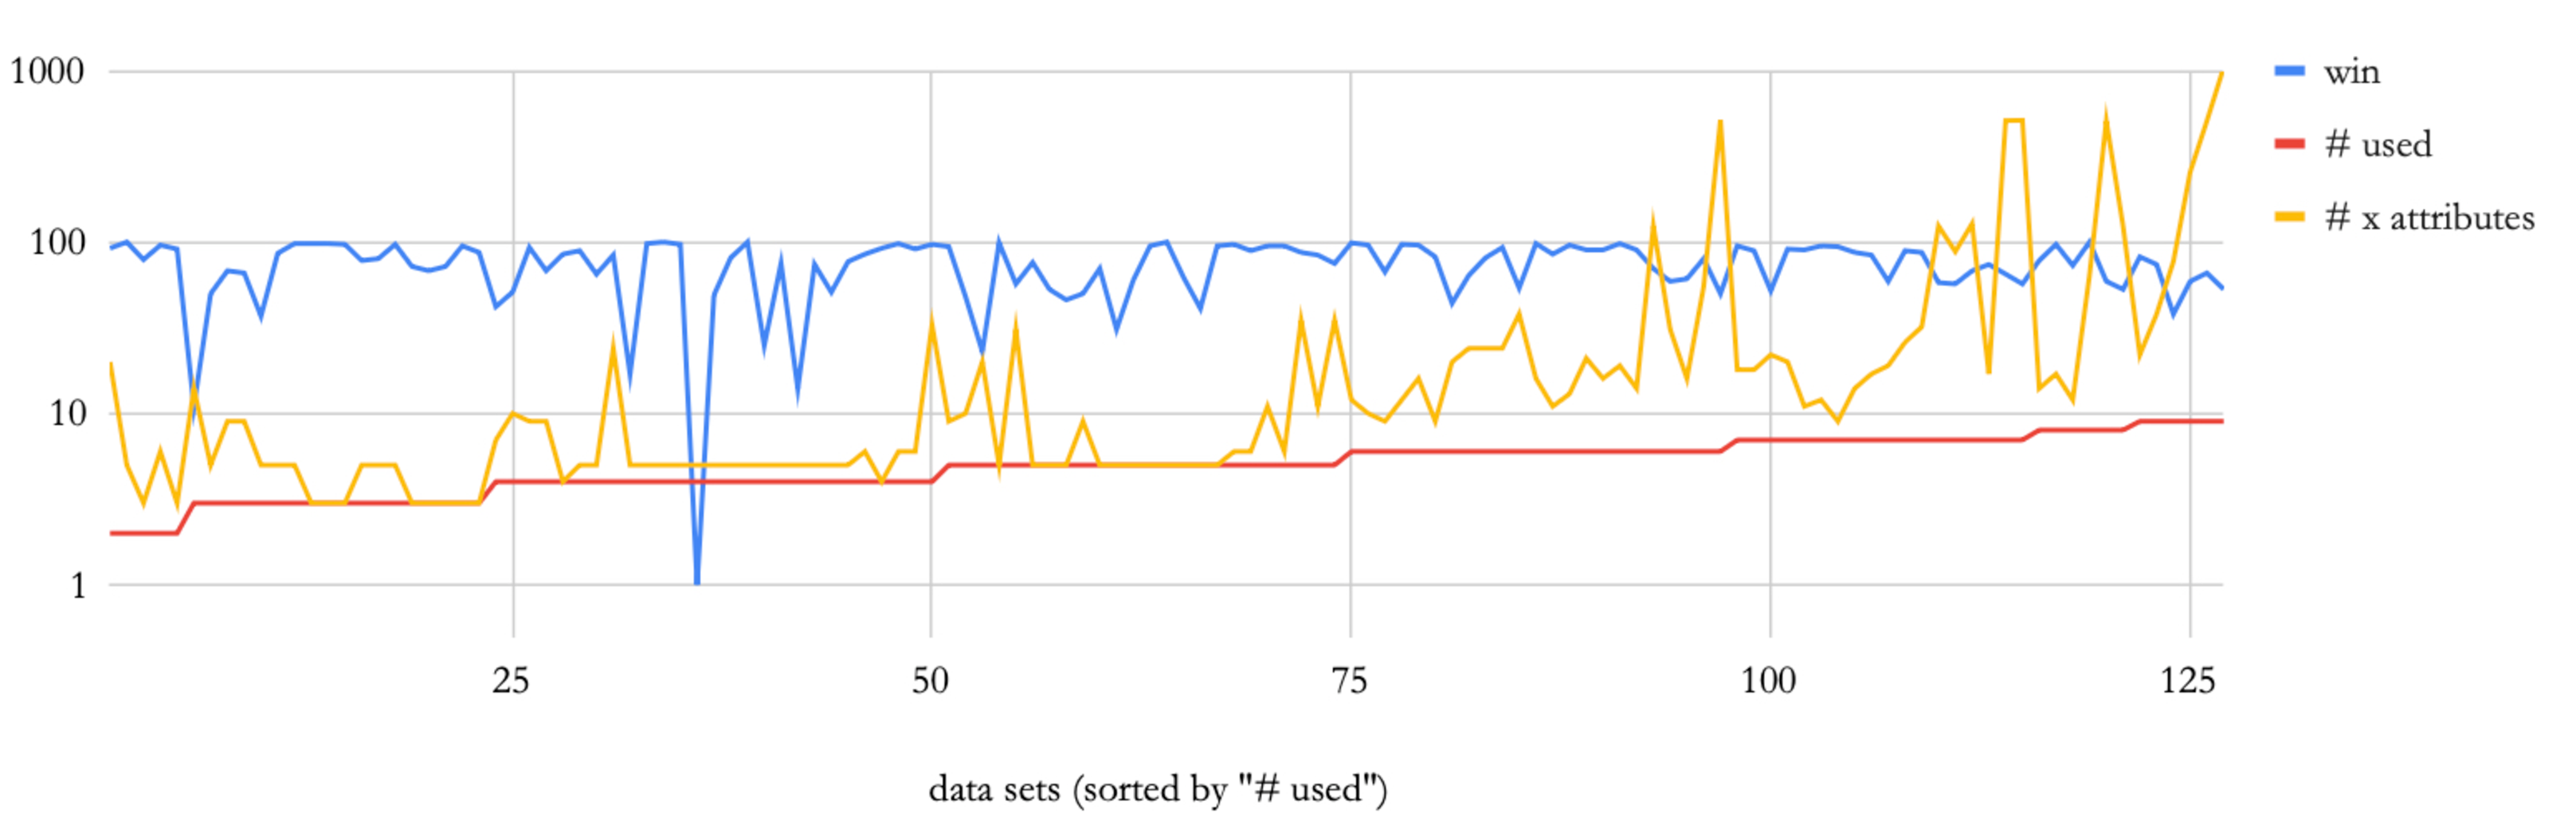
\includegraphics[width=.9\linewidth]{used.pdf}
\end{center}
\caption{Across 120-plus MOOT tasks, the
\color{darkyellow}{\bf yellow line}\color{black}~shows the
number of $x$ attributes available (rising to over a thousand).
The \color{red}{\bf red line}\color{black}~shows the number of
unique attributes \IT{}'s trees actually used (under ten,
throughout). The \color{blue}{\bf blue line}\color{black}~shows
the \textsf{wins} score (\S\ref{sec:using}) of those trees,
hovering near 100 across the entire range. The blue line does
not slope downward as available attributes grow.}
\label{used}
\end{figure*}

This is not a one-off. Figure~\ref{used} shows the same
measurement across all 120-plus MOOT tasks. Three lines:

\begin{itemize}
\item The \color{darkyellow}{\bf yellow line}\color{black}~ is
the number of $x$ attributes available in each task. It rises
from a few dozen to over a thousand as we move right across
MOOT.
\item The \color{red}{\bf red line}\color{black}~ is the number
of unique attributes that actually appear in any of the trees
\IT{} grew on each task. It stays under ten throughout.
\item The \color{blue}{\bf blue line}\color{black}~ is the
\textsf{wins} score (\S\ref{sec:using}) of those trees. It
hovers near 100 across the entire range.
\end{itemize}

The blue line does not slope downward as we move right. Tasks
with thousands of available attributes get scored just as well
by trees with under ten attributes as tasks with a handful of
attributes do. The available column count does not predict the
useful column count.

\begin{hence}{The Small Data Effect}
On the 120-plus MOOT tasks, fewer than ten variables suffice to
build effective predictive models, even when the data set
contains hundreds or thousands of attributes.
\end{hence}

We did not invent this observation. Pearson described principal
components in 1902~\cite{pca}. Chang showed in 1974 that a
handful of exemplar rows can replace a full nearest-neighbor
training set without loss of classification
accuracy~\cite{chang74}. Johnson and Lindenstrauss proved in
1984 that high-dimensional data can be projected to far fewer
dimensions while preserving pairwise
distances~\cite{johnson1984extensions}. Kohavi and John reported
in 1997 that 80\% of features can usually be
discarded~\cite{kohavi97}. Zhu's 2005 semi-supervised learning
survey describes high-dimensional data as typically lying on a
much lower-dimensional manifold~\cite{zhu2005semi}. Settles
argued in 2009 that an active learner querying only the most
informative rows can match a learner trained on the full
set~\cite{settles2009active}. Our own work on SE ``keys'' across
2003--2021 found that a handful of parameters governs the
behavior of many software
models~\cite{me03a,me07a,me21a,menzies2008implications}.

What is new in \IT{} is that the small-data effect extends to
multi-objective optimization. Most of the prior work cited above
was about classification or regression. \IT{} grows trees that
predict \textsf{disty}, which means the trees are doing
multi-objective ranking. The same effect (under ten variables
suffice) holds in that setting too.

\subsection{Comparison with state-of-the-art XAI}

A small tree is not just compact. It is also competitive as an
explanation.

Amirali et al.~\cite{amirali} compared \IT{}'s trees against
SHAP, LIME, and Anchors on standard XAI benchmarks. The metrics
were actionability (does the explanation tell you what to
change?) and faithfulness (does following the explanation
actually move the prediction?). \IT{}'s trees matched or
exceeded the named baselines on both metrics.

The structural difference is worth flagging. SHAP and LIME
approximate a black-box model with a local linear surrogate.
Anchors approximates with rule predicates. \IT{}'s trees do not
approximate. The tree {\em is} the model the active learner
built. There is nothing to be unfaithful to. The tree describes
itself.

This is a useful property in safety-relevant settings. A
practitioner reading a SHAP report cannot easily tell whether
the surrogate has departed from the underlying model. Reading a
\IT{} tree, the practitioner is reading the actual decision
boundary. If the tree says \texttt{pcap == vh} buys 49\% effort
reduction, then \texttt{pcap == vh} buys 49\% effort reduction.

\subsection*{The lesson: the small-data effect, again}

Two findings landed at once. Trees on MOOT use under ten
variables across the board. Those trees match or beat
SHAP/LIME/Anchors on actionability and faithfulness.

The two findings are connected. SHAP and LIME exist because the
underlying model is a black box. \IT{}'s tree is small enough
that nothing is being explained from the outside; the model
explains itself. The cognitive bias toward additive
complexity~\cite{adams2021people} predicts that a researcher
faced with a hard prediction problem will reach for a heavier
model. The MOOT data say the heavier model is rarely required.

% --- end of section ---

\section{Validation: Does the Model Travel?}\label{sec:valid}

The previous section showed that \IT{}'s trees use few
variables and explain themselves well. That is interesting only
if the trees also predict accurately. A small tree built on 30
labels is not useful if it fits the training labels and falls
over on new rows.

This section is the held-out test.

\subsection{Train versus test}

The validation rig in \texttt{ezr.py} is called
\textsf{test\_acquire}. It splits each MOOT data set in half.
The first half (capped at \textsf{the.few} = 128 rows) goes to
the active learner as the training pool. The second half is
hidden, and never touched during acquisition.

\begin{minted}{python}
def ready(file):
  d = (file if Data == type(file)
       else Data(csv(file)))
  random.shuffle(d.rows)
  half = len(d.rows) // 2
  return (d, clone(d, d.rows[:half][:the.few]),
             d.rows[half:])
\end{minted}

\textsf{test\_acquire} runs 20 repeats per setting. Each repeat:
shuffle the data, give the first half to the active learner,
let it spend its budget, grow a tree from the labeled rows, and
score the result two ways.

\begin{minted}{python}
the.learn.check  = 5    # config
the.learn.budget = 30   # config

def test_acquire(file=egopt1):
  d0 = Data(csv(file))
  w1, w2 = Num(), Num()
  win = wins(d0)
  for _ in range(20):
    d, d_train, test_rows = ready(d0)
    lab = acquire(d_train)
    t   = treeGrow(d_train, lab.rows)
    guess = sorted(test_rows,
      key=lambda r: mid(treeLeaf(t, r).ynum))
    add(w1, win(min(
      lab.rows[:the.learn.check],
      key=lambda r: disty(d_train, r))))
    add(w2, win(min(
      guess[:the.learn.check],
      key=lambda r: disty(d_train, r))))
\end{minted}

The two scores answer two different questions.

\textsf{w1} is the train view. Sort the labels the active
learner acquired by their known \textsf{disty}, take the top
\textsf{check}, return the best of those, score with
\textsf{wins}. This asks: how good is the model on rows it has
seen?

\textsf{w2} is the test view. Sort the held-out rows by the tree's
predicted \textsf{disty}, take the top \textsf{check}, return
the best of those, score with \textsf{wins}. This asks: does the
model travel?

\textsf{check} is the small follow-up budget the engineer is
willing to spend after deployment. Five oracle calls is realistic.

\subsection{The Budget--Check trade-off}

Figure~\ref{check} sweeps both budgets. We ran 100,000 trials
across MOOT, drawing \textsf{Budget} uniformly from $[1, 150]$
and \textsf{Check} uniformly from $[1, 10]$. Each cell of the
heatmap is the median \textsf{wins} at that
(\textsf{Budget}, \textsf{Check}) pair, averaged across all
runs that landed there. A small Gaussian blur over neighboring
cells smooths the noise.\footnote{Cells $c_1, c_2, c_3$ at
distance 1, 2, 3 in any direction contribute weights
$(71 c_1 + 25 c_2 + 4 c_3)/100$.}

\begin{figure*}
\begin{center}
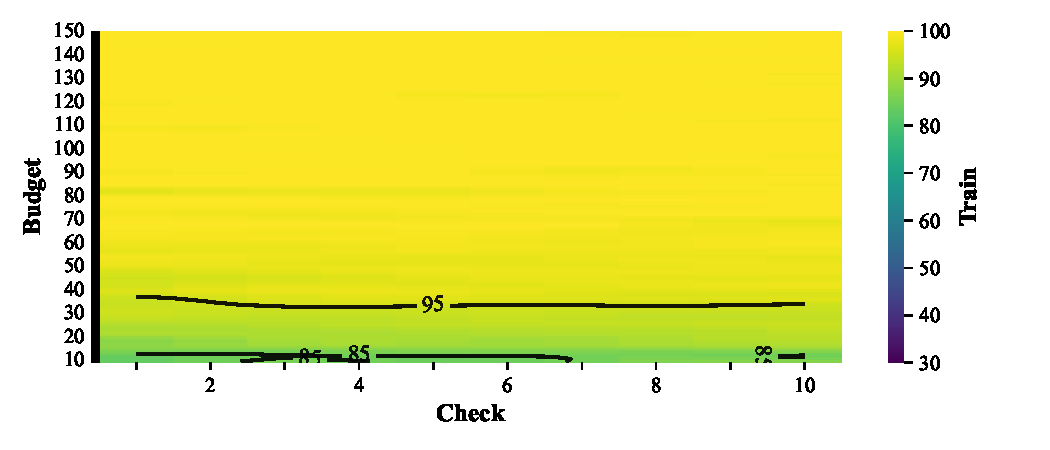
\includegraphics[width=5in]{train.pdf}\\
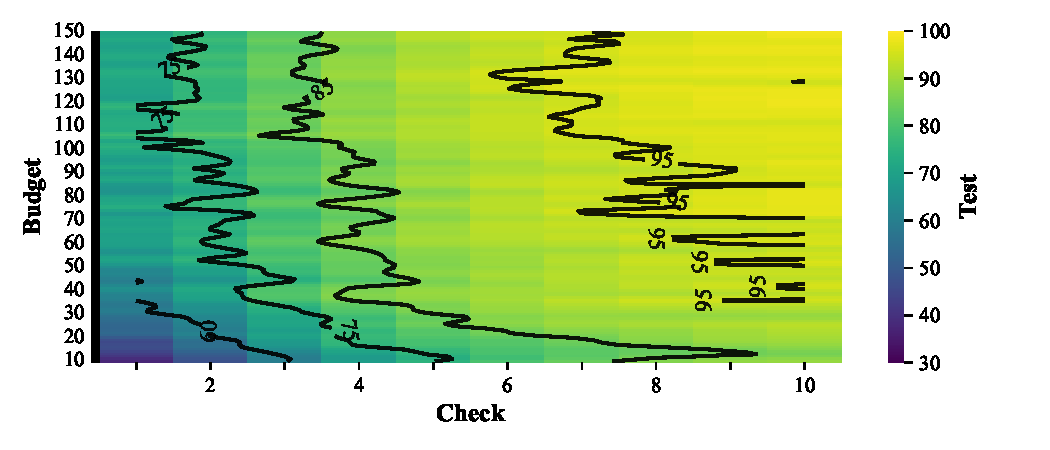
\includegraphics[width=5in]{test.pdf}
\end{center}
\caption{Median \textsf{wins} score as a function of
acquisition \textsf{Budget} (rows) and check budget
\textsf{Check} (columns). {\bf Top:} performance scored on
the training labels (\textsf{w1}); the model is being asked
about rows it built itself from. {\bf Bottom:} performance
scored on held-out test rows ranked by the learned tree
(\textsf{w2}). Contour lines mark \textsf{wins} of 60, 70,
80, 90, 95. Each cell aggregates the median over many trials
at that (\textsf{Budget}, \textsf{Check}) pair, smoothed by a
small Gaussian blur over neighboring cells. Contours flatten
toward the upper right, indicating diminishing returns from
larger budgets.}
\label{check}
\end{figure*}

The top panel reports \textsf{w1} (train). The bottom panel
reports \textsf{w2} (test).

The train panel is forgiving. \textsf{wins} reaches 95
nearly everywhere. This is unsurprising. The model is being
asked about rows it built itself from.

The test panel is the interesting one. The tree is being asked
to rank rows it has never seen.

The picture is encouraging. With a deployment-side budget of 4
to 7 oracle calls, the tree reaches 85--95\% of the reference
optimum across most of the heatmap. The contour lines flatten
toward the upper right. Pushing \textsf{Budget} past 50--100
buys very little. The cost of optimization is dominated by the
small initial labeling phase. After that, a handful of test-time
checks does the rest.

\subsection*{The lesson: a two-phase economy}

The shape of the heatmap mirrors the economics of larger AI
systems.

A pre-trained LLM costs hundreds of millions of dollars to
train. Downstream users then spend a few cents per query
nudging conditional probabilities with in-context examples. The
training cost is amortized; the per-query cost is small.

\IT{}'s training cost is 50 to 100 labels of the active
learner's choosing. Its per-query cost is 4 to 7 oracle calls
on held-out rows. Neither cost is enormous. The shape is the
same as the LLM economy: build the model once, reuse it
cheaply.

The difference is the absolute cost. An LLM costs
$10^{12}$ tokens of training data and runs on a data center.
\IT{} costs 50 labels and runs on a laptop. The shape is shared.
The scale is not.

\section{Case Study: Light-Weight Relevance Filtering}\label{sec:textmine}

The previous sections covered classification, clustering,
optimization, regression-tree explanation, and active learning.
This section is a single case study showing what happens when we
point the same machinery at a problem from a different domain:
text mining.

\subsection{The relevance problem}

Modern AI systems often use Retrieval-Augmented Generation, or
RAG~\cite{lewis2020retrieval}, to answer questions about a
document collection. RAG has two halves. The first finds
documents relevant to a query. The second feeds those documents
to an LLM, which writes the answer.

The first half is an old problem. Given a corpus and a query,
return the documents that match. Modern implementations use
dense neural embeddings (BERT, sentence-transformers, OpenAI's
embedding APIs). Older approaches used active learning with
classical classifiers. The active-learning approaches predate
the embedding approaches and, in some domains, still beat them
on cost.

Yu et al.~\cite{yu2018finding} studied this problem in 2018 in a
particularly painful instance: primary study selection for
systematic literature reviews in software engineering. An SLR
conductor starts with a search query that returns thousands of
papers, of which a few dozen are actually relevant. Reading
every candidate takes weeks or months~\cite{kitchenham2010,
carver2013}. Yu's tool, FASTREAD, used a linear SVM with
uncertainty sampling to early candidates and certainty sampling
later. It reached 95\% recall on Yu's four corpora after labeling
roughly 300--800 papers out of 1,700--8,900. That was a
20--50\% improvement over the prior state of the
art~\cite{wallace2010,miwa2014,cormack2014}.

We asked: can \IT{}'s substrate, plus TWCNB (Rennie et al.,
2003~\cite{rennie2003}), do the same thing in fewer lines?

\subsection{TWCNB on \IT{}'s substrate}

TWCNB is the four-trick refinement of Naive Bayes that closes
the gap to SVMs on text classification. Each of the four tricks
is short, and three of the four ride on the substrate.

\begin{enumerate}
\item Estimate per-word weights from each class's
{\em complement} (rows {\em not} in the class) rather than the
class itself. This corrects bias when class sizes are very
skewed, which they are here: ``relevant'' is 1--2\% of the
corpus.
\item L1-normalize the per-class weight vectors. Rennie's
intent was to keep classes with stronger word dependencies from
dominating.
\item Replace raw term frequencies with $\log(1 + f)$. Real text
follows a power-law (``bursty'') distribution, not the
multinomial that Naive Bayes assumes.
\item Down-weight common terms by inverse document frequency.
\end{enumerate}

The implementation reuses the substrate. Each class is a
\cls{Data}. The per-word weights live in the \cls{Sym} columns
inside that \cls{Data}. \textsf{add} maintains the term
frequencies as papers are labeled. The complement weights are
computed from the union of {\em other} classes via \textsf{sub}.
The full TWCNB scoring code is around 30 lines.

\subsection{Datasets, metrics, and rig}

Yu's four corpora come from real published SE SLRs. Each was
reverse-engineered from the source paper's search query and
inclusion list. The datasets are named after the lead authors
of the source SLRs.

\begin{table}[!t]
\caption{Yu's four SLR corpora~\cite{yu2018finding}. Each is a
search-engine query result where a small minority of candidates
are relevant. The Kitchenham corpus has two relevance levels:
132 papers passed title-and-abstract review, of which 45
survived content review.}
\label{slr}
\begin{center}
\footnotesize
\begin{tabular}{lrr}
\hline
Dataset & \#Candidate & \#Relevant \\
\hline
Wahono       & 7002 & 62 \\
Hall         & 8911 & 104 \\
Radjenovi\'c & 6000 & 48 \\
Kitchenham   & 1704 & 45 (132) \\
\hline
\end{tabular}
\end{center}
\end{table}

The four sources are: Hall et al.~\cite{hall2012} on fault
prediction, Wahono~\cite{wahono2015} on defect prediction,
Radjenovi\'c et al.~\cite{radjenovic2013} on software fault
metrics, and Kitchenham et al.~\cite{kitchenham2010} on a
tertiary review of SLR practice.

We track two metrics from the IR literature.

\textit{Recall} is $\mathit{tp}/(\mathit{tp} + \mathit{fn})$:
the fraction of truly relevant papers found. Higher is better.
The Yu-style target is 95\%.

\textit{False alarm} (sometimes called pf, the false positive
rate) is $\mathit{fp}/(\mathit{fp} + \mathit{tn})$: the fraction
of irrelevant papers incorrectly returned as relevant. Lower is
better.

Yu reported only recall. Reporting recall alone hides how much
irrelevant reading the user still has to do. We report both.

The rig: warm-start with 25 randomly drawn papers, train TWCNB,
add one paper at a time chosen by certainty sampling (the
unlabeled paper TWCNB ranks most strongly as ``yes''), retrain,
re-score. Median and IQR over 20 repeats. Acquisition stops at
95\% recall or budget exhaustion.

We ran two configurations. {\bf Non-normalized} skips Rennie's
L1 normalization; the other three tricks remain.
{\bf Normalized} keeps all four tricks, exactly as TWCNB
recommends.

\begin{figure*}[!t]
\centering
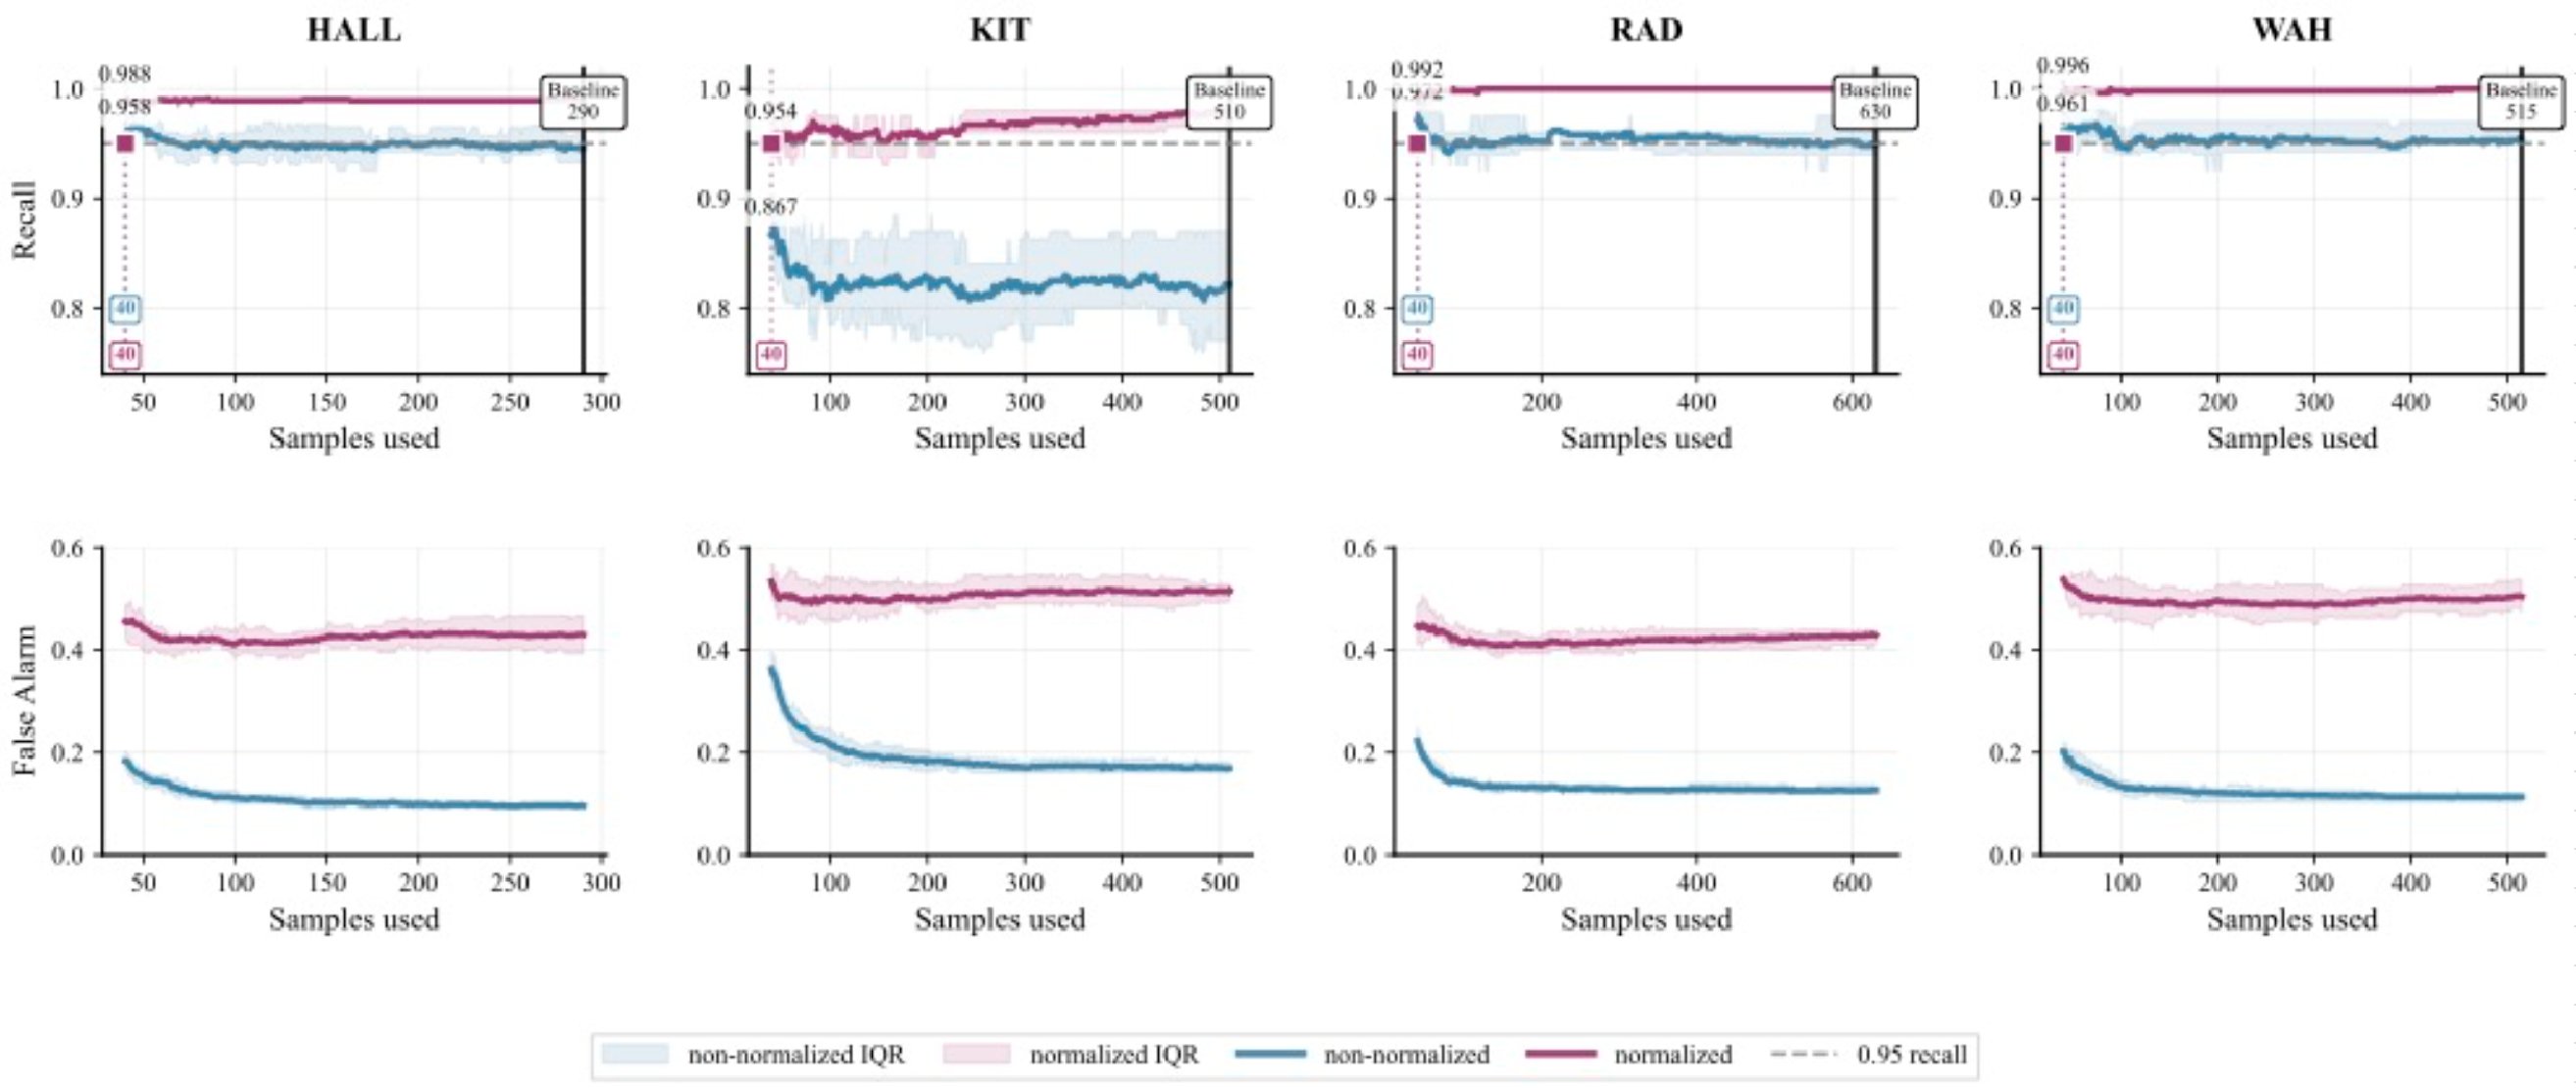
\includegraphics[width=\linewidth]{kit.pdf}
\caption{Recall (top row) and false alarm (bottom row) as a
function of labels acquired, for non-normalized TWCNB (blue)
and normalized TWCNB (red) on Yu's four SLR corpora. Warm-start
= 25 for all runs. Each curve is the median over 20 repeats,
with shaded IQR. Vertical bars on the recall panels mark the
labeling budget at which Yu et al.~\cite{yu2018finding} reached
the same recall with FASTREAD. Numerical labels at the left
edge of each recall panel mark the recall achieved
immediately after the warm start.}
\label{slrfig}
\end{figure*}

\subsection{Results}

Figure~\ref{slrfig} shows recall and false alarm for both
configurations on all four datasets.


Three things stand out.

First, on Hall, Radjenovi\'c, and Wahono, non-normalized TWCNB
reaches 95\% recall right after the warm start. The recall
curves are flat across the rest of the budget. Forty labels are
enough on three of four corpora. FASTREAD needed 290--630.

Second, normalization (red) helps recall slightly but hurts
false alarm a lot. Non-normalized false alarms sit at 10--20\%.
Normalized false alarms sit at 40--50\%. A user following
Rennie's literal recipe ends up reading 4--5 times more
irrelevant papers than necessary. Rennie's L1 normalization
helped on the original 20 Newsgroups / Reuters / Industry Sector
benchmarks. It does not help here. We could only see this
because we measured false alarm. Yu did not.

Third, Kitchenham is the awkward case. On the strict 45-paper
relevance label, recall plateaus around 85\%, well below the
95\% target. But Kitchenham has two relevance levels. The looser
132-paper label includes papers that passed title-and-abstract
review but failed content review. At 82\% recall on the 132-paper
label, TWCNB still finds about 108 relevant papers and misses
fewer than 25. For an SLR conductor whose goal is ``find me
many relevant papers, fast,'' that is still useful. And again:
40 labels.

\subsection*{The lesson: half of RAG, in 30 lines}

Compared to Yu's FASTREAD, \IT{}+TWCNB:

\begin{itemize}
\item uses fewer labels (40 vs. 290--630) on three of four
corpora;
\item uses a simpler classifier (Naive Bayes vs. linear SVM);
\item uses a smaller codebase (around 30 lines of TWCNB plus a
small driver, riding on the substrate);
\item reports both recall {\em and} false alarm, surfacing that
one of TWCNB's recommended tricks is counterproductive in this
domain. Yu's study could not have found this because Yu reported
only recall.
\end{itemize}

This last point is the methodological one. Re-running prior
work with simple methods is not just a way to compress the code.
It is a way to revisit prior measurements. Yu's data was fine.
The choice of metrics was incomplete. The simpler tool exposed
the gap.

The retrieval task TWCNB does here is half of what RAG does.
The other half is dialog generation, which is genuinely the LLM
half. We are not arguing LLMs are unnecessary. We are arguing
that a non-trivial fraction of what RAG pipelines do can be
done by methods that pre-date the deep-learning revolution,
when those methods are built on a substrate that makes them
small.

The cognitive bias toward additive complexity~\cite{adams2021people}
shows up here too. It is easier to add a vector database than
to ask whether one is needed. Trying the simple thing first
costs almost nothing. Sometimes it ends the investigation.

% --- end of section ---

\section{Discussion: Is Simple Also Stupid?}\label{sec:disc}

We started with a question. Five lessons in, with three
empirical comparisons on the table, this is where we answer it.

\subsection{The five lessons, in light of the evidence}

The introduction listed five lessons. We can now check each one
against what the body of the paper showed.

\textit{Many models can be tiny.} Across 120-plus MOOT tasks,
trees with under ten variables matched or beat heavier
explanation tools (\S\ref{sec:tiny}, citing Amirali et
al.~\cite{amirali}).

\textit{Random search works better than expected.} On MOOT, the
(1+1)-EA, simulated annealing, and local search were
statistically indistinguishable. They differed only in a one-line
accept rule (\S\ref{sec:opt}).

\textit{One data structure suffices.} Naive Bayes, $k$-means,
$k$-means++, three optimizers, the active learner, and TWCNB all
sit on the same \cls{Num}/\cls{Sym}/\cls{Data} substrate
(\S\ref{sec:peek} through \S\ref{sec:textmine}).

\textit{Optimization, classification, and regression are nearly
the same algorithm.} The textbook gives them separate chapters.
The code gives them five sections of the same source file
(\S\ref{sec:famous}, \S\ref{sec:opt}, \S\ref{sec:active}).

\textit{Small codebases work.} \IT{} is around 500 lines, with
no heavy dependencies. The active learner runs 10{,}000 times
faster than SMAC~\cite{kashin}. The text-mining classifier runs
in milliseconds on a laptop (\S\ref{sec:textmine}).

Three independent comparisons, three domains, the same pattern.
Simple, when carefully built, is not stupid.

\subsection{Where simple genuinely fails}

\IT{} is not a universal substitute. There are real tasks for
which no simple method we know of works.

Generation is the clearest case. Translation, summarization,
code synthesis, and natural-language interfaces require an
understanding of language that no \cls{Num}/\cls{Sym} substrate
can carry. The training data and compute budget that build LLMs
are not bypass-able for these tasks.

Dense perception is another. Image classification at scale,
speech recognition under noise, and protein structure prediction
have all moved decisively to large neural models. Smaller
methods exist but lose on benchmarks that matter.

Tasks with strong sequential dependencies are a third case.
Sequence-to-sequence problems where context windows of thousands
of tokens carry meaning are not what \IT{} is designed for.

What \IT{} is good at is structured tabular data with explicit
$x$ and $y$ columns where the $y$ column is expensive to
compute. That covers a lot of SE: configuration tuning, defect
prediction, hyperparameter search, test selection, cost
estimation, and (as the case study showed) some text mining
problems too. It does not cover everything.

\subsection{The cognitive bias toward additive complexity}

The simplification we found in \IT{} was not invisible. It was
in the code. We had to read it.

Adams et al.~\cite{adams2021people} document a robust cognitive
bias: people, when given a problem, tend to add new components
rather than remove existing ones. The bias survives when
subtraction is the better choice and when the addition has a
cost. \IT{} is the product of repeatedly subtracting. We removed
multi-generational genetic algorithms in favor of one-generation
sampling. We removed adaptive active learning samplers in favor
of greedy search. We removed pandas in favor of 14 lines of CSV
parsing. We removed regression tree ensembles in favor of two
\cls{Data}s.

A survey by Hou et al.~\cite{Hou24} of 229 SE papers using LLMs
found that only 5\% baselined against non-LLM alternatives.
That is the additive bias at scale: the field reaches for the
heavy method without checking whether the light one would have
worked. When checked, the light method often does
work~\cite{grinsztajn2022why,somvanshi2024survey,Tawosi23,
majumder2018500+,Ling24,Fu17,johnson2024ai}.

\IT{} is one demonstration. We do not claim it generalizes
beyond SE multi-objective optimization, classification, and the
relevance-filtering case study. We do claim that within those
boundaries, the simpler tool kept reaching state-of-the-art
results, and the simpler tool exposed gaps in prior measurement
that the heavier tools missed.

\subsection{Threats to validity}

\textit{Construct.} ``State of the art'' depends on the metric.
We compared on actionability and faithfulness for explanations
(following Amirali et al.~\cite{amirali}); on solution quality
under fixed budgets for optimization (following
Ganguly~\cite{kashin}); on recall and false alarm for relevance
filtering. Different metrics could give different results. We
chose metrics that were either standard in the prior work or
(in the relevance case) more complete than the prior work.

\textit{Internal.} Active learning is stochastic. We report
medians over 20 repeats with IQR shading throughout. Larger
repeat counts might reveal smaller effects. The 100,000-trial
heatmap in \S\ref{sec:valid} is one defense against this.

\textit{External.} Our comparisons rest on MOOT (120-plus SE
tasks) and Yu's four SLR corpora. Generalization beyond these
data sets is an open question. SE is itself a limited domain;
results may not transfer to other application areas.

\textit{Conclusion.} The headline claim that \IT{} ``matches
state of the art'' uses Cliff's-delta plus
Kolmogorov--Smirnov tests for statistical sameness. Like any
tied-or-better claim, this allows that another study could
report a clear win for the heavier method. We have not seen
such a study, but we cannot rule it out.

\subsection{Conclusion}

We started with the question {\em is simple also stupid?}\
Across MOOT, across Yu's SLR corpora, and across the
explanation comparisons of Amirali et al., the answer was no.

The simplification was not in the algorithms. The algorithms in
\IT{} are textbook. The simplification was in noticing that
five textbook algorithms shared one data structure, and writing
the data structure once.

That noticing took years of reading and rewriting code.
It cannot happen in a workflow that treats the code as something
the AI emits and the human consumes. It happens when the human
sits with the code, deletes things, and watches what survives.
The 500 lines of \IT{} are what survived.

If the field continues toward methods that are large and
opaque, this paper is a vote in the other direction. The simple
thing is worth trying first. It often works. When it does, the
code fits on the page.

\appendix
\section{Building and Displaying Trees}\label{app:trees}
# Tree Growth and Use

EZR's regression trees are built {\em after} active learning is done.
The {\em best}/{\em rest} machinery in \textsf{acquire} (line~\ref{s1})
collected a small set of labeled rows; \textsf{treeGrow} now distills
those rows into a readable rule set that predicts \textsf{disty}.

A \cls{Tree} node holds the rows that fell to it (in a child \cls{Data}
called \textsf{d}), a summary \cls{Num} of their \textsf{disty} values
(\textsf{ynum}), and---if the node has split---the chosen column,
cut value, and two children:
\begin{minted}{python}
class Tree: 
  def __init__(i, data, rows):
    i.d = clone(data, rows)
    i.ynum=adds((disty(data,row) for row in rows),Num())
    i.col,i.cut = None,0
    i.left=i.right=None
\end{minted}
\textsf{treeCuts} proposes split points for one column. For symbols,
all distinct values are candidates; for numbers, just the median (a
deliberate simplification that keeps trees small and fast):
\begin{minted}{python}
def treeCuts(col, rows): 
  vs=[row[col.at] for row in rows if row[col.at]!="?"]
  if not vs: return []
  return (set(vs) if Sym == type(col)
          else [sorted(vs)[len(vs)//2]])
\end{minted}

\textsf{treeSplit} evaluates one (column, cut) pair by partitioning
the rows and scoring the result by weighted \textsf{spread} of
\textsf{disty}---the same \textsf{spread} function defined earlier
(standard deviation for \cls{Num}s, entropy for \cls{Sym}s). Lower
scores mean tighter, more predictable leaves:
\begin{minted}{python}
def treeSplit(data, col, cut, rows): 
  l_rows,r_rows,l_num,r_num=[],[],Num(),Num()
  for row in rows:
    v = row[col.at]
    go=v=="?" or (v==cut if Sym==type(col) else v<=cut)
    (l_rows if go else r_rows).append(row)
    add(l_num if go else r_num,disty(data,row))
  s=l_num.n*spread(l_num)+r_num.n*spread(r_num)
  return s,col,cut,l_rows,r_rows
\end{minted}

\textsf{treeGrow} ties it together: enumerate every (column, cut)
pair from the $x$ columns, keep splits where both sides have at
least \textsf{the.learn.leaf} rows, take the lowest-spread split,
and recurse. The recursion stops when too few rows remain to split
further:
\begin{minted}{python}
def treeGrow(data, rows): 
  tree = Tree(data, rows)
  if len(rows) >= 2 * the.learn.leaf:
    splits = (treeSplit(data, col, cut, rows)
              for col in tree.d.cols.xs
              for cut in treeCuts(col, rows))
    if valid := [s for s in splits
        if min(len(s[3]),len(s[4]))
           >= the.learn.leaf]:
      _, tree.col, tree.cut, left, right = min(
        valid, key=lambda x: x[0])
      tree.left  = treeGrow(data, left)
      tree.right = treeGrow(data, right)
  return tree
\end{minted}

That is the entire builder. Note what is {\em not} here: no entropy
gain, no Gini, no pruning pass, no surrogate splits, no bagging.
\textsf{spread} already handles both numeric and symbolic targets
(by polymorphism on \textsf{col} type), so one routine covers what
CART and C4.5 split into many. The deliberate restriction to the
median cut for numeric columns means \textsf{treeGrow} considers
$O(|\textit{xs}|)$ splits per node rather than $O(|\textit{xs}| \cdot
|\textit{rows}|)$; on the small label sets EZR works with, this is
both fast and surprisingly effective.

\smallskip

Once the tree exists, three small functions use it.
\textsf{treeLeaf} routes a row to its leaf by walking the splits
(missing values fall right, by convention):
\begin{minted}{python}
def treeLeaf(tree, row): 
  if not tree.left: return tree
  v = row[tree.col.at]
  go = v!="?" and (v<=tree.cut
    if Num==type(tree.col) else v==tree.cut)
  return treeLeaf(tree.left if go else tree.right,row)
\end{minted}

\textsf{treeNodes} is a depth-first generator that yields every node
along with its level, the column/op/cut that led to it, and---when a
node has children---visits them sorted by \textsf{mid(ynum)} so that
the most promising branch (lowest \textsf{disty}) is shown first. This
sort is what makes printed trees like Figure~\ref{htree} read
top-to-bottom from best to worst:
\begin{minted}{python}
def treeNodes(tree,lvl=0,col=None,op="",cut=None): 
  yield tree, lvl, col, op, cut
  if tree.col:
    ops=("<=",">") if Num==type(
      tree.col) else ("==","!=")
    kids=sorted([(tree.left,ops[0]),
      (tree.right,ops[1])],
      key=lambda z:mid(z[0].ynum))
    for k, txt in kids:
      if k: yield from treeNodes(k,lvl+1,
        tree.col,txt,tree.cut)
\end{minted}

\textsf{treeShow} consumes that generator to print the tree. Each
line carries the indented split, the leaf's mean \textsf{disty}, the
row count, and the per-goal \textsf{mid} values---which is exactly
the format of Figure~\ref{htree}, where the gap between rows
\rc{1} and \rc{2} revealed the 43\% productivity win:
\begin{minted}{python}
def treeShow(tree): 
  for t1,lvl,col,op,cut in treeNodes(tree):
    p=f"{col.txt} {op} {o(cut)}" if col else ""
    if lvl > 0: p = "|   "*(lvl-1) + p
    g={col.txt:mid(col) for col in t1.d.cols.ys}
    print(f"{p:<{the.show.show}}"
          f",{o(mid(t1.ynum)):>4}"
          f" ,({t1.ynum.n:3}), {o(g)}")
\end{minted}
% Finally, \textsf{treePlan} turns the tree into {\em counterfactual
% advice}. Given the leaf where a row currently sits (\textsf{here}),
% it walks every other leaf and yields those with meaningfully lower
% \textsf{disty}---``meaningfully'' meaning beyond a small-effect
% threshold (Sawilowsky's $0.35\sigma$, the same threshold used in
% \textsf{wins} at line~\ref{wins}). For each such leaf, it reports
% which $x$ columns would need to change and to what:
% \begin{minted}{python}
% def treePlan(tree, here): 
%   eps = the.stats.eps * spread(tree.ynum)
%   for there,_,_,_,_ in treeNodes(tree):
%     if there.col is None and \
%       (dy:=mid(here.ynum)-mid(there.ynum))>eps:
%       diff=[f"{col.txt}={o(mid(col))}"
%         for col,h in zip(there.d.cols.xs,here.d.cols.xs)
%         if mid(col) != mid(h)]
%       if diff:
%         yield dy, mid(there.ynum), diff
% \end{minted}

% This is what makes EZR's trees more than predictors. They are
% {\em advisors}: they not only score a configuration but tell the
% engineer what to change to reach a better one---and silently
% report which $x$ variables never appeared in any split, which is
% how Figure~\ref{used} could conclude that fewer than ten variables
% matter even on 1000-variable data.


\bibliography{bib3,main}
\end{document}